%Version 3.1 December 2024
% See section 11 of the User Manual for version history
%
%%%%%%%%%%%%%%%%%%%%%%%%%%%%%%%%%%%%%%%%%%%%%%%%%%%%%%%%%%%%%%%%%%%%%%
%%                                                                 %%
%% Please do not use \input{...} to include other tex files.       %%
%% Submit your LaTeX manuscript as one .tex document.              %%
%%                                                                 %%
%% All additional figures and files should be attached             %%
%% separately and not embedded in the \TeX\ document itself.       %%
%%                                                                 %%
%%%%%%%%%%%%%%%%%%%%%%%%%%%%%%%%%%%%%%%%%%%%%%%%%%%%%%%%%%%%%%%%%%%%%

%%\documentclass[referee,sn-basic]{sn-jnl}% referee option is meant for double line spacing

%%=======================================================%%
%% to print line numbers in the margin use lineno option %%
%%=======================================================%%

%%\documentclass[lineno,pdflatex,sn-basic]{sn-jnl}% Basic Springer Nature Reference Style/Chemistry Reference Style

%%=========================================================================================%%
%% the documentclass is set to pdflatex as default. You can delete it if not appropriate.  %%
%%=========================================================================================%%

%%\documentclass[sn-basic]{sn-jnl}% Basic Springer Nature Reference Style/Chemistry Reference Style

%%Note: the following reference styles support Namedate and Numbered referencing. By default the style follows the most common style. To switch between the options you can add or remove �Numbered� in the optional parenthesis. 
%%The option is available for: sn-basic.bst, sn-chicago.bst%  
 
%%\documentclass[pdflatex,sn-nature]{sn-jnl}% Style for submissions to Nature Portfolio journals
%%\documentclass[pdflatex,sn-basic]{sn-jnl}% Basic Springer Nature Reference Style/Chemistry Reference Style
\documentclass[pdflatex,sn-mathphys-ay]{sn-jnl}% Math and Physical Sciences Numbered Reference Style
%%\documentclass[pdflatex,sn-mathphys-ay]{sn-jnl}% Math and Physical Sciences Author Year Reference Style
%%\documentclass[pdflatex,sn-aps]{sn-jnl}% American Physical Society (APS) Reference Style
%%\documentclass[pdflatex,sn-vancouver-num]{sn-jnl}% Vancouver Numbered Reference Style
%%\documentclass[pdflatex,sn-vancouver-ay]{sn-jnl}% Vancouver Author Year Reference Style
%%\documentclass[pdflatex,sn-apa]{sn-jnl}% APA Reference Style
%%\documentclass[pdflatex,sn-chicago]{sn-jnl}% Chicago-based Humanities Reference Style

%%%% Standard Packages
%%<additional latex packages if required can be included here>

\usepackage{graphicx}%
\usepackage{multirow}%
\usepackage{amsmath,amssymb,amsfonts}%
\usepackage{amsthm}%
\usepackage{mathrsfs}%
\usepackage[title]{appendix}%
\usepackage{xcolor}%
\usepackage{textcomp}%
\usepackage{manyfoot}%
\usepackage{booktabs}%
\usepackage{algorithm}%
\usepackage{algorithmicx}%
\usepackage{algpseudocode}%
\usepackage{listings}%
%%%%

%%%%%=============================================================================%%%%
%%%%  Remarks: This template is provided to aid authors with the preparation
%%%%  of original research articles intended for submission to journals published 
%%%%  by Springer Nature. The guidance has been prepared in partnership with 
%%%%  production teams to conform to Springer Nature technical requirements. 
%%%%  Editorial and presentation requirements differ among journal portfolios and 
%%%%  research disciplines. You may find sections in this template are irrelevant 
%%%%  to your work and are empowered to omit any such section if allowed by the 
%%%%  journal you intend to submit to. The submission guidelines and policies 
%%%%  of the journal take precedence. A detailed User Manual is available in the 
%%%%  template package for technical guidance.
%%%%%=============================================================================%%%%

%% as per the requirement new theorem styles can be included as shown below
\theoremstyle{thmstyleone}%
\newtheorem{theorem}{Theorem}%  meant for continuous numbers
%%\newtheorem{theorem}{Theorem}[section]% meant for sectionwise numbers
%% optional argument [theorem] produces theorem numbering sequence instead of independent numbers for Proposition
\newtheorem{proposition}[theorem]{Proposition}% 
%%\newtheorem{proposition}{Proposition}% to get separate numbers for theorem and proposition etc.

\theoremstyle{thmstyletwo}%
\newtheorem{example}{Example}%
\newtheorem{remark}{Remark}%

\theoremstyle{thmstylethree}%
\newtheorem{definition}{Definition}%

\raggedbottom
%%\unnumbered% uncomment this for unnumbered level heads

\begin{document}

\title{Adaptive-OCGCN: Ambiguity-Aware Overlap Assignment for Scalable Graph Neural Networks}

%%=============================================================%%
%% GivenName	-> \fnm{Joergen W.}
%% Particle	-> \spfx{van der} -> surname prefix
%% FamilyName	-> \sur{Ploeg}
%% Suffix	-> \sfx{IV}
%% \author*[1,2]{\fnm{Joergen W.} \spfx{van der} \sur{Ploeg} 
%%  \sfx{IV}}\email{iauthor@gmail.com}
%%=============================================================%%

\author*[1,2]{\fnm{Mahmood} \sur{Amintoosi}}\email{m.amintoosi@um.ac.ir}

\affil[1]{\orgdiv{Computer Science Division, Department of Applied Mathematics, Faculty of Mathematical Sciences}, \orgname{Ferdowsi University of Mashhad}, \orgaddress{
%\street{Street}, 
\city{P. O. Box 1159, Mashhad 91775}, %\postcode{100190}, \state{State}, 
\country{Iran}}}

\affil[2]{\orgdiv{Graph Theory and its Applications Lab.}, \orgname{Faculty of Mathematical Sciences, Ferdowsi University of Mashhad},  \orgaddress{
%\street{Street}, 
\city{Mashhad}, 
%\postcode{10587}, \state{State},
 \country{Iran}}}

%%==================================%%
%% Sample for unstructured abstract %%
%%==================================%%

\abstract{Graph Convolutional Networks (GCNs) have demonstrated strong performance on graph learning tasks, but their scalability remains challenging for large-scale graphs.
Cluster-based training approaches, such as Cluster-GCN, address this issue by partitioning large graphs into smaller subgraphs; however, hard partitioning may discard important inter-cluster information.
Overlapping Cluster-GCN (OCGCN) alleviates this limitation by allowing boundary nodes to participate in multiple clusters through overlap assignment.
Nevertheless, OCGCN relies on a fixed global Winner Membership Closeness (WMC) threshold, which requires dataset-specific tuning and does not consider the uncertainty of individual node memberships.

In this work, we propose Adaptive-OCGCN, an ambiguity-aware overlap assignment framework that replaces global thresholding with node-specific adaptive decisions.
The proposed approach exploits community-membership ambiguity to identify nodes whose assignments are inherently uncertain.
Specifically, we introduce three adaptive strategies: Entropy-Adaptive WMC, which utilizes normalized membership entropy, Margin-Adaptive WMC, which measures ambiguity through the gap between the two most likely community memberships, and Hybrid-Adaptive WMC, which combines both signals.

We evaluate the proposed methods on six benchmark graph datasets (Cora, CiteSeer, PubMed, ACM, DBLP, and IMDB) using multiple random seeds and compare them with fixed-threshold OCGCN baselines.
The results demonstrate that adaptive overlap assignment matches tuned fixed-threshold OCGCN while removing the need for dataset-specific WMC grid search.
Across 20 seeds and six datasets, Margin-Adaptive WMC outperforms the untuned default threshold on four of six datasets, with a significant pooled paired gain, and adaptive methods also improve performance on four of six datasets at comparable overlap ratios.
Furthermore, ambiguity analysis shows that high-entropy nodes contain 41--95\% overlap candidates, whereas low-entropy nodes contain only 0--17\%, confirming that membership uncertainty provides a meaningful criterion for overlap selection.
Overall, Adaptive-OCGCN provides a practical and principled approach for scalable graph neural network training by integrating uncertainty-aware overlap assignment into partition-based learning.}

%%================================%%
%% Sample for structured abstract %%
%%================================%%

% \abstract{\textbf{Purpose:} The abstract serves both as a general introduction to the topic and as a brief, non-technical summary of the main results and their implications. The abstract must not include subheadings (unless expressly permitted in the journal's Instructions to Authors), equations or citations. As a guide the abstract should not exceed 200 words. Most journals do not set a hard limit however authors are advised to check the author instructions for the journal they are submitting to.
% 
% \textbf{Methods:} The abstract serves both as a general introduction to the topic and as a brief, non-technical summary of the main results and their implications. The abstract must not include subheadings (unless expressly permitted in the journal's Instructions to Authors), equations or citations. As a guide the abstract should not exceed 200 words. Most journals do not set a hard limit however authors are advised to check the author instructions for the journal they are submitting to.
% 
% \textbf{Results:} The abstract serves both as a general introduction to the topic and as a brief, non-technical summary of the main results and their implications. The abstract must not include subheadings (unless expressly permitted in the journal's Instructions to Authors), equations or citations. As a guide the abstract should not exceed 200 words. Most journals do not set a hard limit however authors are advised to check the author instructions for the journal they are submitting to.
% 
% \textbf{Conclusion:} The abstract serves both as a general introduction to the topic and as a brief, non-technical summary of the main results and their implications. The abstract must not include subheadings (unless expressly permitted in the journal's Instructions to Authors), equations or citations. As a guide the abstract should not exceed 200 words. Most journals do not set a hard limit however authors are advised to check the author instructions for the journal they are submitting to.}

\keywords{Graph Convolutional Networks, Overlapping Clustering, Cluster-GCN, Membership Ambiguity, Adaptive Thresholding}

%%\pacs[JEL Classification]{D8, H51}

%%\pacs[MSC Classification]{35A01, 65L10, 65L12, 65L20, 65L70}

\maketitle

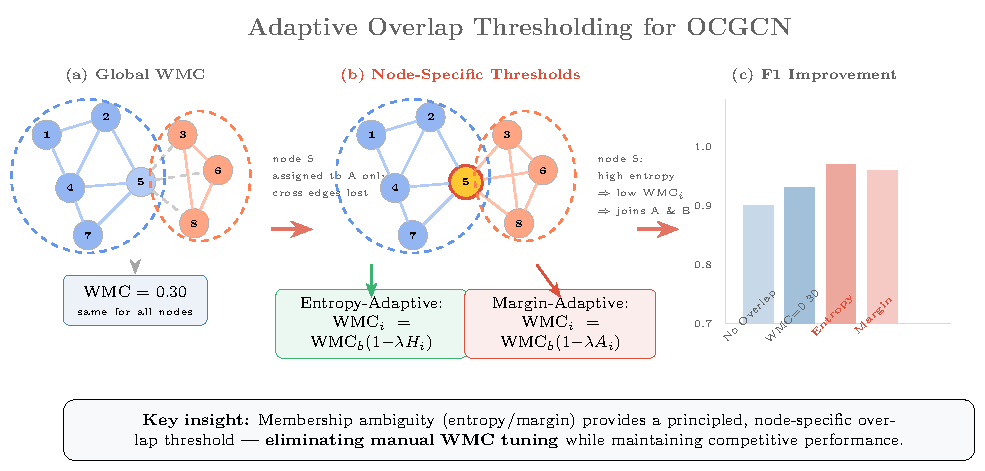
\includegraphics[width=1\linewidth]{graphical_abstract.pdf}

\tableofcontents

%%======================================================================
\section{Introduction}
\label{sec:introduction}
%%======================================================================

Graph Convolutional Networks (GCNs) have become a foundational tool for semi-supervised node classification on graph-structured data~\citep{kipf2017semi}.
However, applying GCNs to large-scale graphs remains challenging due to neighborhood explosion, where each convolutional layer requires aggregating information from increasingly large neighborhoods, resulting in substantial memory and computational costs~\citep{Cluster-GCN}.
To address this issue, Cluster-GCN partitions a large graph into smaller subgraphs and performs mini-batch training on these clusters, achieving improved scalability while preserving most local graph structures~\citep{Cluster-GCN}.
The underlying assumption is that nodes within the same partition contain sufficient structural information and that the loss of cross-cluster dependencies is limited.

Nevertheless, real-world graphs often exhibit overlapping community structures, where individual nodes naturally participate in multiple semantic or structural groups.
For example, papers in citation networks may connect multiple research areas, while entities in heterogeneous networks may simultaneously play different roles.
When traditional partitioning assigns such boundary nodes exclusively to a single cluster, important cross-community information may be discarded, leading to incomplete node representations.

Overlapping Cluster-GCN (OCGCN), introduced in our earlier study~\citep{Amintoosi2021}, was an initial attempt to incorporate overlapping community membership into partition-based GCN training.
Specifically, OCGCN employs a non-negative matrix factorization based community detection method (DANMF) to obtain soft community memberships and allows nodes with significant membership in multiple clusters to participate in multiple cluster subgraphs.
This overlap mechanism enables the GCN model to access richer structural contexts during training.

Despite its effectiveness, OCGCN determines overlap membership using a single global Winner Membership Closeness (WMC) threshold.
Such a global decision rule assumes that all nodes exhibit similar levels of community certainty, which is rarely true in real-world networks.
A node with nearly uniform membership across several communities represents a highly ambiguous case, whereas a node with one dominant community and a weak secondary membership has a substantially different structural meaning.
However, both nodes are treated identically under a fixed global threshold.
Furthermore, the appropriate WMC value varies across datasets, requiring additional hyperparameter tuning and limiting the practicality of overlap-aware training.

In this work, we introduce \textit{Adaptive-OCGCN}, an ambiguity-aware overlap assignment framework that replaces the fixed global overlap criterion with node-specific adaptive decisions.
The central idea is that community-membership ambiguity provides a natural signal for identifying nodes that benefit most from multi-cluster participation.
We propose three complementary adaptive strategies: \textit{Entropy-Adaptive WMC}, which uses normalized membership entropy to identify nodes with distributed community affiliations, \textit{Margin-Adaptive WMC}, which exploits the gap between the two largest membership probabilities to detect nodes located near community boundaries, and \textit{Hybrid-Adaptive WMC}, which combines both signals.
All strategies preserve the original OCGCN formulation while introducing node-level adaptivity through an ambiguity-aware adjustment mechanism.

Unlike previous overlap-aware approaches that treat overlap selection as a global partitioning decision, Adaptive-OCGCN formulates overlap assignment as a node-level uncertainty-aware learning problem.
The main contributions of this work are summarized as follows:

\begin{enumerate}
  \item We identify a fundamental limitation of existing overlap-aware Cluster-GCN training: fixed global overlap criteria ignore node-level variation in community-membership ambiguity.
  
  \item We propose \textit{Adaptive-OCGCN}, an ambiguity-aware overlap assignment framework with three adaptive strategies, Entropy-Adaptive WMC, Margin-Adaptive WMC, and their Hybrid combination, which derive node-specific overlap decisions from membership uncertainty.
  
  \item We demonstrate through extensive experiments on six benchmark graph datasets that adaptive overlap assignment achieves competitive or improved performance compared with fixed-threshold OCGCN while substantially reducing dataset-specific WMC tuning.
  
  \item We perform a detailed ambiguity analysis showing that membership uncertainty strongly correlates with overlap suitability, providing empirical evidence that ambiguity is a principled criterion for selecting nodes for overlapping training.
\end{enumerate}

%%======================================================================
\section{Related Work}
\label{sec:related}
%%======================================================================

This section surveys three lines of research relevant to our work: scalable graph neural network training (Section~\ref{subsec:clustergcn}), overlapping community detection and soft membership modeling (Section~\ref{subsec:danmf}), and overlap-aware partition-based training (Section~\ref{subsec:ocgcn}).
We also review recent advances in adaptive and uncertainty-aware graph learning (Section~\ref{subsec:ambiguity}) and motivate our ambiguity-based approach.

\subsection{Scalable Graph Neural Network Training}

Graph Convolutional Networks (GCNs) have become a fundamental approach for representation learning on graph-structured data by iteratively aggregating information from neighboring nodes~\citep{kipf2017semi}.
However, applying GCNs to large-scale graphs remains challenging due to the neighborhood explosion problem, where multi-layer message passing requires accessing exponentially increasing neighborhoods.

Several approaches have been proposed to improve the scalability of GNN training.
GraphSAGE~\citep{GraphSAGE} and FastGCN~\citep{chen2018fastgcn} reduce computational costs through neighborhood sampling, while VR-GCN~\citep{dai2018learning} introduces variance reduction techniques by reusing historical node representations.
Although sampling-based approaches improve efficiency, they may introduce approximation errors and remain challenging for very deep architectures.

Cluster-GCN~\citep{Cluster-GCN} follows a different strategy by partitioning a large graph into smaller clusters and performing mini-batch training on cluster-induced subgraphs.
By restricting message passing within each partition, Cluster-GCN significantly reduces memory and computational requirements while maintaining competitive performance.
However, this approach relies on a hard partitioning assumption: nodes are assigned to a single cluster, and cross-cluster interactions are largely ignored.
Consequently, nodes located near community boundaries may lose important structural information during training.

\subsection{Overlapping Community Learning and Soft Membership Modeling}

Many real-world networks exhibit overlapping community structures, where individual nodes simultaneously participate in multiple semantic or structural groups.
Unlike traditional hard clustering methods, overlapping community detection approaches aim to learn soft membership representations that capture the degree of association between nodes and communities.

Existing overlapping community detection methods include clique-based approaches, label propagation techniques, and matrix factorization based methods~\citep{Shang2014}.
Non-negative matrix factorization (NMF) methods represent each node using a membership vector over latent communities.
Deep Adversarial Non-negative Matrix Factorization (DANMF)~\citep{DANMF} extends this idea by combining deep autoencoding and adversarial learning to obtain informative community representations.

Recent studies have further explored graph neural network based approaches for overlapping community discovery.
He et al.~\citep{He2022} proposed a semi-supervised overlapping community detection framework using graph convolutional autoencoders.
Yuan et al.~\citep{Yuan2022} investigated overlapping community detection using graph convolutional networks on complex networks.
UCoDe~\citep{UCoDe2023} introduced a unified graph convolutional framework for community detection, while Li et al.~\citep{Li2023} proposed a dual graph neural network architecture for overlapping community detection.
Sismanis et al.~\citep{Sismanis2024} further explored graph attention networks for identifying overlapping communities.

Although these approaches effectively model overlapping community structures, their primary objective is community discovery.
They do not consider how overlapping memberships can be exploited to improve scalable graph neural network training under partition-based learning frameworks.

\subsection{Overlap-Aware Partition-Based GNN Training}

While most previous studies have investigated overlapping communities for network analysis and community discovery, Overlapping Cluster-GCN (OCGCN)~\citep{Amintoosi2021} introduced a different perspective by utilizing overlapping memberships to improve scalable graph neural network training.

OCGCN extends Cluster-GCN by incorporating soft community memberships obtained from DANMF into the graph partitioning process.
Instead of assigning every node to a single cluster, OCGCN allows nodes with significant memberships in multiple communities to participate in multiple cluster subgraphs.
This strategy alleviates the information loss caused by hard partitioning and provides richer structural contexts for GCN training.

The overlap assignment in the original OCGCN framework is controlled by a Winner Membership Closeness (WMC) threshold.
A node is assigned to cluster $c$ if its membership value satisfies:

\[
P(i,c) \geq \mathrm{WMC}\cdot \max_{c'}P(i,c').
\]

Although this mechanism improves boundary-node representation, it applies the same global threshold to all nodes.
Such a criterion assumes that all nodes have similar levels of community certainty, while real-world graphs contain both highly confident nodes and highly ambiguous nodes with competing community memberships.
Therefore, overlap selection in OCGCN remains dependent on dataset-specific threshold tuning rather than node-level structural characteristics.

\subsection{Adaptive and Uncertainty-Aware Graph Learning}

Adaptive mechanisms have recently attracted increasing attention in graph representation learning.
Graph Attention Networks (GAT)~\citep{vel2018graph}, for example, learn node-specific importance coefficients to dynamically control information aggregation.
Similarly, adaptive neighborhood selection approaches adjust message-passing structures according to graph topology and learning objectives~\citep{Peng2021, Guang2024}.

Beyond adaptive aggregation, uncertainty-aware learning has emerged as an important direction for understanding model reliability and decision confidence.
Gawlikowski et al.~\citep{Gawlikowski2023} provided a comprehensive survey of uncertainty estimation methods in deep neural networks, highlighting the importance of uncertainty modeling for reliable prediction.
Several graph learning studies have also incorporated confidence-aware mechanisms for improving robustness and reliability~\citep{Kwon2022, Park2023}.

However, existing adaptive and uncertainty-aware graph learning approaches mainly focus on message aggregation, neighborhood selection, or prediction reliability.
They do not address the problem of deciding which nodes should participate in multiple graph partitions during scalable GNN training.

In this work, we bridge this gap by introducing membership ambiguity as a node-level uncertainty signal for overlap assignment.
Unlike previous approaches that treat overlap selection as a global partitioning decision, Adaptive-OCGCN formulates overlap assignment as an uncertainty-aware node-level learning problem.

\subsection{Cluster-GCN}
\label{subsec:clustergcn}

Cluster-GCN~\citep{Cluster-GCN} accelerates GCN training by exploiting graph partitioning.
Given a graph $\mathcal{G}=(\mathcal{V},\mathcal{E})$ with $N=|\mathcal{V}|$ nodes, Cluster-GCN partitions $\mathcal{V}$ into $K$ disjoint clusters $\{C_1,\ldots,C_K\}$.

Instead of performing full-batch training on the entire graph, a GCN is trained on cluster-induced subgraphs $\mathcal{G}[C_k]$, where message passing is restricted to nodes within each cluster.
This reduces memory consumption and computational complexity, making GCN training feasible for large-scale graphs.

The standard GCN layer is defined as:

\begin{equation}
H^{(l+1)}
=
\sigma
\left(
\tilde{D}^{-\frac{1}{2}}
\tilde{A}
\tilde{D}^{-\frac{1}{2}}
H^{(l)}
W^{(l)}
\right),
\label{eq:gcn-layer}
\end{equation}

where $\tilde{A}=A+I_N$ represents the adjacency matrix with self-loops, $\tilde{D}$ is the corresponding degree matrix, $W^{(l)}$ is a trainable weight matrix, and $\sigma$ denotes the activation function.

The main assumption of Cluster-GCN is that most important structural information is preserved within clusters.
However, when nodes lie at the intersection of multiple communities, removing cross-cluster connections may lead to incomplete neighborhood information and degraded representations.

\subsection{Overlapping Cluster-GCN}
\label{subsec:ocgcn}

Overlapping Cluster-GCN (OCGCN)~\citep{Amintoosi2021} extends Cluster-GCN by relaxing the assumption of disjoint graph partitions.
The main idea is to identify boundary nodes with significant memberships in multiple communities and allow them to participate in multiple cluster subgraphs.

The OCGCN framework consists of four main steps:

\begin{enumerate}

\item {Soft Community Assignment.}
A community detection algorithm based on DANMF produces a soft membership matrix
$P\in\mathbb{R}^{N\times K}$,
where $P(i,c)$ indicates the membership strength of node $i$ in cluster $c$.

\item {Overlap Assignment.}
For each node $i$, OCGCN selects clusters satisfying:

\begin{equation}
P(i,c)\geq \mathrm{WMC}\times\max_{c'}P(i,c').
\label{eq:wmc}
\end{equation}

where $\mathrm{WMC}\in(0,1]$ is the Winner Membership Closeness threshold.

\item {Overlapping Subgraph Construction.}
Nodes selected for multiple clusters are duplicated across corresponding cluster subgraphs while preserving their original features and labels.

\item {Training and Prediction.}
Independent GCN models are trained on cluster subgraphs.
For overlapping nodes, predictions from multiple assigned clusters are aggregated.

\end{enumerate}

By allowing boundary nodes to appear in multiple partitions, OCGCN reduces the information loss caused by hard graph partitioning.
However, the original framework uses a single global WMC threshold for all nodes.
This ignores the fact that membership distributions may have different levels of certainty, motivating an adaptive overlap assignment strategy.

\subsection{Soft Community Membership and DANMF}
\label{subsec:danmf}

DANMF~\citep{DANMF} is a deep adversarial non-negative matrix factorization method that learns latent community representations.
Unlike hard clustering, DANMF provides soft membership vectors, allowing each node to have different association strengths with multiple communities.

The resulting normalized membership matrix is denoted by
$P\in\mathbb{R}^{N\times K}$,
where:

\begin{equation}
P(i,c)\geq0,
\qquad
\sum_{c=1}^{K}P(i,c)=1.
\end{equation}

These membership distributions provide the foundation for measuring node-level community ambiguity in our adaptive overlap assignment framework.

\subsection{Community Membership Ambiguity}
\label{subsec:ambiguity}

The central hypothesis of this work is that nodes with uncertain community memberships are more suitable candidates for overlap assignment.
To quantify this uncertainty, we consider two complementary measures derived from the membership distribution $P(i,:)$.

\paragraph{Normalized Entropy.}

Entropy measures the global uncertainty of the membership distribution:

\begin{equation}
H_{\mathrm{norm}}(i)
=
\frac{
-\sum_{c=1}^{K}P(i,c)\log P(i,c)
}
{\log K}.
\label{eq:entropy}
\end{equation}

A value close to zero indicates a concentrated membership distribution, where one community dominates.
A value close to one indicates that the node has similar memberships across communities.

\paragraph{Membership Margin Ambiguity.}

Entropy captures uncertainty across all communities, but it does not specifically focus on competition between the most likely communities.
Therefore, we additionally define a margin-based ambiguity score:

\begin{equation}
A(i)=1-(p_1-p_2),
\label{eq:ambiguity}
\end{equation}

where $p_1$ and $p_2$ denote the largest and second-largest membership values of node $i$.

A small margin between the two dominant communities indicates that the node lies near a community boundary.
Thus, high values of $A(i)$ correspond to nodes with ambiguous cluster assignments.

Entropy and margin ambiguity capture different aspects of uncertainty.
Entropy measures the overall distribution spread, whereas margin ambiguity focuses on the competition between the two strongest communities.
These complementary characteristics motivate the two adaptive overlap assignment strategies proposed in this work.
%%======================================================================
\section{Proposed Method}
\label{sec:method}
%%======================================================================

Given a graph
$\mathcal{G}=(\mathcal{V},\mathcal{E})$
with node features
$X\in\mathbb{R}^{N\times d}$
and labels
$Y$ for a subset of nodes, the objective of semi-supervised node classification is to learn a graph neural network model that predicts labels for unlabeled nodes.
For large-scale graphs, Cluster-GCN addresses the computational challenge by partitioning the graph into $K$ disjoint subgraphs.
However, hard partitioning may remove important cross-community interactions, especially for nodes located near community boundaries.
OCGCN alleviates this limitation by introducing an overlapping partitioning mechanism.
Given a soft community membership matrix

\begin{equation}
P\in\mathbb{R}^{N\times K},
\end{equation}

where $P(i,c)$ denotes the membership strength of node $i$ in community $c$, OCGCN determines the cluster assignments of each node using a global Winner Membership Closeness threshold:

\begin{equation}
\mathcal{C}_i
=
\left\{
c \mid
P(i,c)\geq
\mathrm{WMC}\times
\max_{c'}P(i,c')
\right\}.
\label{eq:ocgcn-assignment}
\end{equation}

Although effective, this formulation applies the same $\mathrm{WMC}$ value to all nodes, which does not consider the confidence of individual community memberships.
For example, a node with an ambiguous membership distribution

\[
P(i,:)=[0.35,0.33,0.32]
\]

and a node with a confident assignment

\[
P(j,:)=[0.90,0.08,0.02]
\]

are processed using the same overlap criterion, despite having fundamentally different structural characteristics.
The problem addressed in this work is therefore to determine node-specific overlap assignments by exploiting membership ambiguity, while preserving the scalability advantages of partition-based GNN training.
More formally, we seek an adaptive overlap assignment function:

\begin{equation}
\mathcal{C}_i=f(P(i,:),\lambda),
\end{equation}

where $f(\cdot)$ determines the cluster participation of node $i$ based on its membership distribution, and $\lambda$ controls the strength of adaptation.
The desired adaptive assignment mechanism should satisfy three properties: ambiguity awareness (nodes with uncertain community memberships should have higher probability of being assigned to multiple clusters), confidence preservation (nodes with dominant memberships should avoid unnecessary overlap), and hyperparameter efficiency (the method should reduce dependence on dataset-specific threshold tuning).

This section introduces our adaptive overlap assignment framework.
Section~\ref{subsec:overview} provides a high-level overview of the adaptive threshold mechanism.
Sections~\ref{subsec:entropy-adaptive}--\ref{subsec:hybrid-adaptive} present three complementary adaptive strategies based on entropy, margin, and hybrid ambiguity signals.
Section~\ref{subsec:comparison} compares these strategies, and algorithm \ref{alg:adaptive} summarizes the complete procedure.

\subsection{Overview}
\label{subsec:overview}

The original OCGCN determines overlap assignments using a single global WMC threshold.
However, nodes in a graph exhibit different levels of community-membership certainty.
Therefore, we reformulate overlap selection as an ambiguity-aware decision process, where each node is assigned an adaptive threshold according to its membership distribution.

Let $a_i \in [0,1]$ denote the ambiguity score of node $i$.
A high value of $a_i$ indicates that the node has uncertain community membership and is a potential boundary node.
The adaptive threshold is defined as:

\begin{equation}
  \mathrm{WMC}_i =
  \max\left(0.01,\ \mathrm{WMC}_{\mathrm{base}}
  \left(1-\lambda a_i\right)\right),
  \label{eq:adaptive}
\end{equation}

where $\mathrm{WMC}_{\mathrm{base}}$ is the reference threshold inherited from the original OCGCN formulation and $\lambda\in[0,1]$ controls the adaptation strength.

When $\lambda=0$, the proposed method reduces to the original OCGCN with a fixed global threshold.
Increasing $\lambda$ allows ambiguous nodes to receive lower thresholds and consequently participate in additional cluster subgraphs.
To avoid excessive overlap, $\mathrm{WMC}_i$ is bounded below by 0.01.
The same lower bound applies to all adaptive variants introduced below.

Using the adaptive threshold, node $i$ is assigned to cluster $c$ if:

\begin{equation}
P(i,c)\geq
\mathrm{WMC}_i
\max_{c'}P(i,c').
\label{eq:selection-rule}
\end{equation}

The proposed framework is independent of the community detection algorithm and can be applied whenever a soft membership matrix is available.
In this work, we use DANMF-generated memberships as the input representation.

\subsection{Entropy-Adaptive WMC}
\label{subsec:entropy-adaptive}

Entropy-Adaptive WMC defines the ambiguity score using the normalized entropy of the membership distribution:

\begin{equation}
a_i = H_{\mathrm{norm}}(i),
\label{eq:entropy-score}
\end{equation}

which results in:

\begin{equation}
\mathrm{WMC}_i =
\max\left(0.01,\ \mathrm{WMC}_{\mathrm{base}}
(1-\lambda H_{\mathrm{norm}}(i))\right).
\label{eq:entropy-adaptive}
\end{equation}

\paragraph{Mechanism.}

Nodes with concentrated membership distributions have low entropy and retain a threshold close to $\mathrm{WMC}_{\mathrm{base}}$.
Consequently, confident nodes are unlikely to be assigned to unnecessary additional clusters.
In contrast, nodes with high entropy distribute their membership probability among several communities and receive a lower threshold, allowing them to participate in multiple cluster subgraphs.

\paragraph{Advantages.}

Entropy considers the complete membership distribution rather than only the two most probable clusters.
Therefore, it is suitable for graphs where nodes may simultaneously relate to multiple communities.
Furthermore, normalization makes the ambiguity score comparable across datasets with different numbers of detected communities.

\subsection{Margin-Adaptive WMC}
\label{subsec:margin-adaptive}

Margin-Adaptive WMC uses the ambiguity derived from the difference between the two largest membership probabilities:

\begin{equation}
a_i=A(i)=1-(p_1-p_2),
\label{eq:margin-score}
\end{equation}

leading to:

\begin{equation}
\mathrm{WMC}_i =
\max\left(0.01,\ \mathrm{WMC}_{\mathrm{base}}
(1-\lambda A(i))\right).
\label{eq:margin-adaptive}
\end{equation}

\paragraph{Mechanism.}

When the largest membership probability is substantially higher than the second largest, the node has a clear community assignment and receives a threshold close to the base value.
When the top two memberships are close, the node represents a community boundary and is assigned a lower threshold to preserve cross-community information.

\paragraph{Advantages.}

Unlike entropy, margin ambiguity focuses specifically on competition between the two dominant communities.
This makes it particularly suitable for graphs where overlapping behavior mainly occurs between pairs of communities rather than across multiple communities.

\subsection{Hybrid-Adaptive WMC}
\label{subsec:hybrid-adaptive}

Hybrid-Adaptive WMC combines the entropy and margin ambiguity signals into a single score:

\begin{equation}
a_i = \max\left(H_{\mathrm{norm}}(i),\ A(i)\right),
\label{eq:hybrid-score}
\end{equation}

leading to:

\begin{equation}
\mathrm{WMC}_i =
\max\left(0.01,\ \mathrm{WMC}_{\mathrm{base}}
\left(1-\lambda \cdot \max\left(H_{\mathrm{norm}}(i),\ A(i)\right)\right)\right).
\label{eq:hybrid-adaptive}
\end{equation}

By taking the maximum of the two complementary ambiguity scores, the hybrid reacts to whichever signal---global distribution spread or top-two competition---is dominant for each node, stays in $[0,1]$, and remains comparable across datasets.

\subsection{Comparison of Adaptive Methods}
\label{subsec:comparison}

Table~\ref{tab:method-comparison} summarizes the characteristics of the three proposed strategies.
	
\begin{table}[ht]
\centering
\caption{Comparison of ambiguity-aware overlap assignment strategies.}
\label{tab:method-comparison}
\begin{tabular}{lccc}
\toprule
\textbf{Aspect} & \textbf{Entropy-Adaptive} & \textbf{Margin-Adaptive} & \textbf{Hybrid-Adaptive} \\
\midrule
Membership information & Full distribution $P(i,:)$ & Top-two memberships & Both signals \\
Ambiguity captured & Global distribution uncertainty & Dominant community competition & Combined \\
Per-node computation & $O(K)$ & $O(K \log K)$ & $O(K \log K)$ \\
Suitable scenario & Multi-community ambiguity & Binary community boundary & General purpose \\
\bottomrule
\end{tabular}
\end{table}

The three strategies capture complementary aspects of membership uncertainty.
Entropy is more appropriate when uncertainty is distributed across several communities, margin ambiguity is more targeted toward nodes located between two dominant communities, and the hybrid combines both signals.
In our experiments the hybrid provides a robust general-purpose configuration, achieving the best result on DBLP.
Algorithm~\ref{alg:adaptive} summarizes the complete adaptive overlap assignment procedure.

\begin{algorithm}[ht]
\caption{Adaptive Overlap Assignment}
\label{alg:adaptive}
\begin{algorithmic}[1]
\Require{Soft membership matrix $P \in \mathbb{R}^{N \times K}$, base threshold $\mathrm{WMC}_{\mathrm{base}}$, adaptation strength $\lambda \in [0,1]$, ambiguity type $\tau \in \{\text{Entropy}, \text{Margin}, \text{Hybrid}\}$}
\Ensure{Adaptive cluster assignments $\mathcal{C}_i$ for all nodes $i = 1, \ldots, N$}
\For{$i \leftarrow 1$ \textbf{to} $N$}
  \If{$\tau = \text{Entropy}$}
    \State{$a_i \leftarrow H_{\mathrm{norm}}(i)$ \Comment{Using Eq.~\eqref{eq:entropy}}}
  \ElsIf{$\tau = \text{Margin}$}
    \State{$a_i \leftarrow 1 - (p_1 - p_2)$ \Comment{Using Eq.~\eqref{eq:ambiguity}}}
  \Else
    \State{$a_i \leftarrow \max\left(H_{\mathrm{norm}}(i),\ A(i)\right)$ \Comment{Using Eq.~\eqref{eq:hybrid-score}}}
  \EndIf
  \State{$\mathrm{WMC}_i \leftarrow \max\left(0.01,\ \mathrm{WMC}_{\mathrm{base}} \times (1 - \lambda a_i)\right)$}
  \State{$p_{\max} \leftarrow \max_{c'} P(i, c')$}
  \State{$\mathcal{C}_i \leftarrow \{c \mid P(i, c) \geq \mathrm{WMC}_i \times p_{\max}\}$}
\EndFor
\State{\Return $\{\mathcal{C}_i\}_{i=1}^{N}$}
\end{algorithmic}
\end{algorithm}

%%======================================================================
\section{Experiments}
\label{sec:experiments}
%%======================================================================

This section describes the experimental setup and presents our results.
We begin with the datasets (Section~\ref{subsec:datasets}) and baseline configurations (Section~\ref{subsec:baselines}).
We then present the main results comparing adaptive methods against fixed-threshold baselines (Section~\ref{sec:results}), including ablation studies, fairness analysis, computational overhead, statistical significance, and an analysis of the relationship between membership ambiguity and overlap quality.

\subsection{Datasets}
\label{subsec:datasets}

We evaluate on six benchmark graphs spanning citation networks and heterogeneous networks.
Table~\ref{tab:datasets} summarizes their characteristics.

\begin{table}[ht]
\centering
\caption{Dataset characteristics.}
\label{tab:datasets}
\begin{tabular}{lrrrr}
\toprule
\textbf{Dataset} & \textbf{Nodes} & \textbf{Edges} & \textbf{Classes} & \textbf{Features} \\
\midrule
Cora & 2,708 & 5,278 & 7 & 1,433 \\
CiteSeer & 3,327 & 4,552 & 6 & 3,703 \\
PubMed & 19,717 & 44,324 & 3 & 500 \\
ACM & 2,363 & 5,318 & 3 & 1,870 \\
DBLP & 2,591 & 3,528 & 4 & 1,433 \\
IMDB & 4,630 & 54,576 & 5 & 1,703 \\
\bottomrule
\end{tabular}
\end{table}

Cora, CiteSeer, and PubMed are citation networks where nodes represent papers and edges represent citation links.
ACM, DBLP, and IMDB are bibliographic or entertainment networks (papers--authors--subjects for ACM and DBLP; movies--actors--directors for IMDB) projected into homogeneous graphs.

\subsection{Baselines}
\label{subsec:baselines}

We compare against three baseline configurations:

\begin{enumerate}
  \item {Cluster-GCN (No Overlap):} Crisp clustering with no overlap nodes, representing the lower bound.
  \item {OCGCN with fixed WMC:} The original OCGCN~\citep{Amintoosi2021} with fixed WMC thresholds of 0.10, 0.20, 0.30, 0.40, and 0.50, representing the upper bound when hyperparameters are tuned.
  \item {Adaptive WMC variants:} Entropy-Adaptive, Margin-Adaptive, and their Hybrid combination with $\lambda \in \{0.25, 0.50, 0.75\}$.
\end{enumerate}

To situate the cluster-based results, we additionally evaluate three standard full-batch architectures --- GCN, GraphSAGE, and GAT --- and a \emph{random-partition} control (the same cluster-based pipeline with random node assignment instead of DANMF). The full-batch models use a comparable architecture to the cluster GCN (16 hidden units per layer, dropout 0.5, Adam lr 0.01) but train on the entire graph with 200 epochs; the random-partition control uses the same per-cluster protocol as the DANMF no-overlap configuration. Table~\ref{tab:standard-baselines} and Figure~\ref{fig:standard-baselines} report micro F1 over 20 seeds.

\begin{table}[ht]
\centering
\caption{Micro F1 (mean~$\pm$~std, 20 seeds) of standard full-batch baselines (200 epochs) and the random-partition control, compared with the best cluster-based method per dataset.}
\label{tab:standard-baselines}
\begin{tabular}{lcccc}
\toprule
\textbf{Dataset} & \textbf{GCN} & \textbf{GraphSAGE} & \textbf{GAT} & \textbf{Random Part.} \\
\midrule
Cora      & \textbf{0.866$\pm$0.011} & 0.861$\pm$0.011 & 0.865$\pm$0.011 & 0.730$\pm$0.016 \\
CiteSeer  & \textbf{0.727$\pm$0.013} & 0.723$\pm$0.013 & 0.727$\pm$0.011 & 0.697$\pm$0.017 \\
PubMed    & 0.865$\pm$0.004 & \textbf{0.883$\pm$0.004} & 0.855$\pm$0.004 & 0.852$\pm$0.004 \\
ACM       & 0.921$\pm$0.010 & \textbf{0.923$\pm$0.007} & 0.923$\pm$0.010 & 0.876$\pm$0.012 \\
DBLP      & 0.848$\pm$0.015 & \textbf{0.853$\pm$0.015} & 0.845$\pm$0.013 & 0.807$\pm$0.014 \\
IMDB      & 0.417$\pm$0.011 & \textbf{0.449$\pm$0.016} & 0.400$\pm$0.015 & 0.374$\pm$0.015 \\
\bottomrule
\end{tabular}
\end{table}

\begin{figure}[ht]
\centering
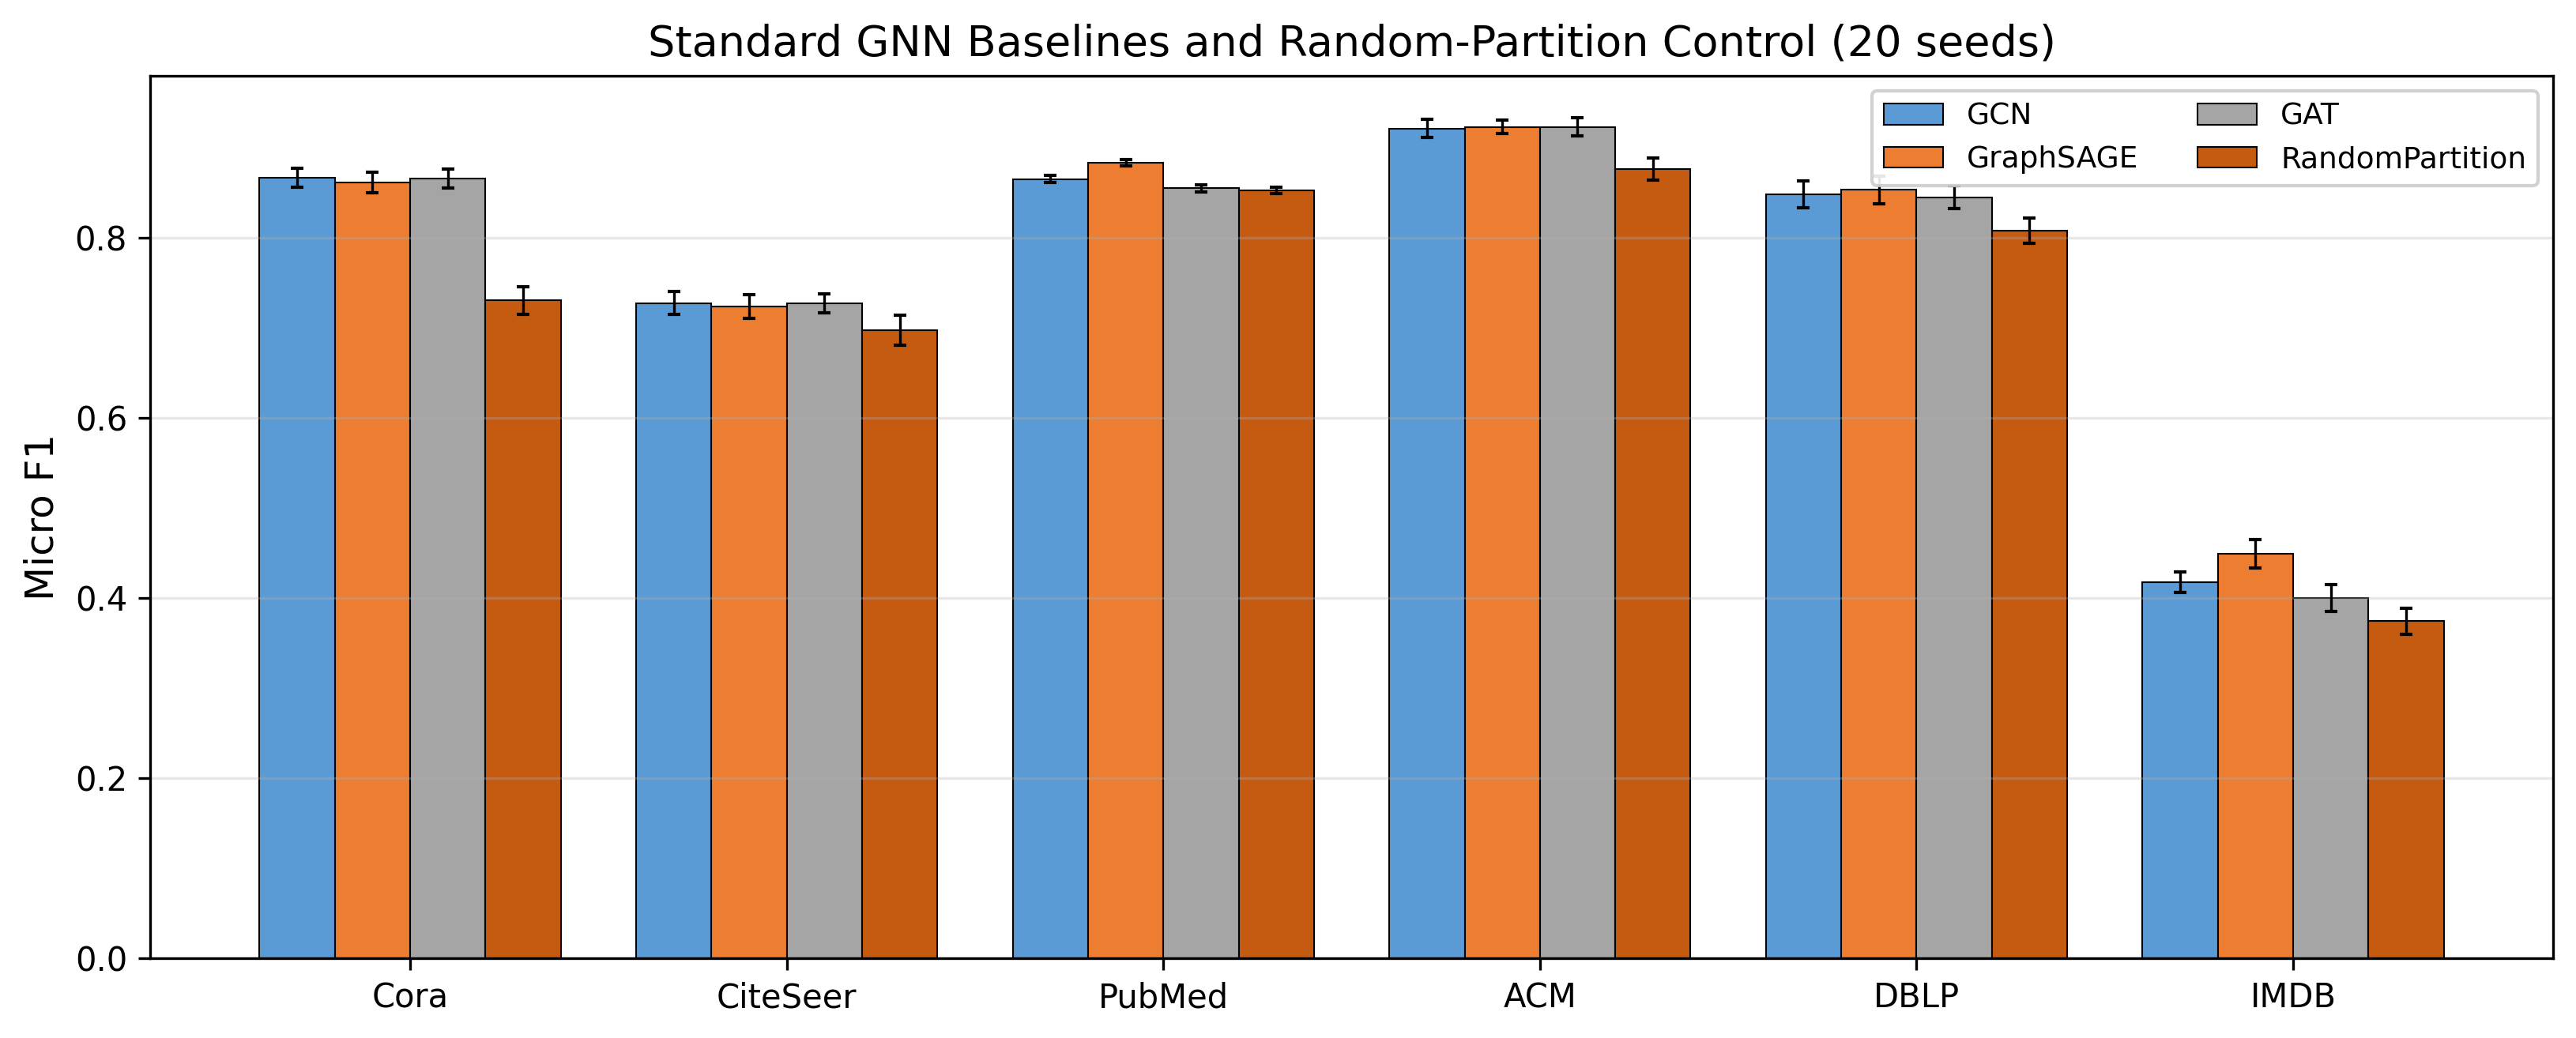
\includegraphics[width=\textwidth]{figures/standard_baselines.png}
\caption{Standard full-batch GNN baselines and the random-partition control (micro F1, 20 seeds, mean~$\pm$~std).}
\label{fig:standard-baselines}
\end{figure}

Two observations follow. First, full-batch training achieves higher accuracy than cluster-based training on most datasets (e.g., Cora 0.866 vs.\ 0.830), which is expected: partition-based training trades a modest amount of accuracy for scalability on large graphs, the motivation of Cluster-GCN itself. Second, the random-partition control reveals that clustering quality matters: on Cora, CiteSeer, ACM, DBLP, and IMDB the DANMF no-overlap baseline (0.798, 0.705, 0.910, 0.829, 0.393) exceeds random assignment (0.730, 0.697, 0.876, 0.808, 0.374). PubMed is the exception: DANMF produces a highly imbalanced partition there (the largest cluster contains about 62\% of the nodes), and the resulting no-overlap score (0.521) falls below the random-partition control (0.852). This is a limitation of the DANMF clustering on PubMed, not of the overlap selection, and it motivates our adaptive methods, which recover substantial F1 on PubMed (0.628) despite the degraded partition. We discuss this in Section~\ref{sec:threats}.

\subsection{Results}
\label{sec:results}

All experiments use:
\begin{itemize}
  \item $\mathrm{WMC}_{\mathrm{base}} = 0.3$
  \item 3-layer GCN with 16 hidden units, ReLU activation, and dropout rate 0.5
  \item Adam optimizer with learning rate 0.01, 10 epochs per subgraph
  \item Train/test split: 70\%/30\% random (per cluster)
  \item 20 random seeds per configuration for the main comparison and 10 for the ablation study; we report micro F1 (macro F1 is also computed)
  \item DANMF for community detection with the number of latent communities set to twice the number of classes per dataset (matching the original OCGCN protocol)
\end{itemize}

The adaptive overlap selection adds negligible computational overhead: entropy and margin computations are $O(K)$ and $O(K \log K)$ per node respectively, applied once after DANMF convergence and before GCN training.
Measured wall-clock training times are reported in Table~\ref{tab:runtime} (NVIDIA RTX 3090, mean over 20 seeds).


\subsubsection{Adaptive vs.\ Global WMC}
\label{subsec:adaptive-vs-global}

Table~\ref{tab:main-results} presents micro-F1 scores for Cluster-GCN (no overlap), original OCGCN (WMC~=~0.30), and the three adaptive methods with $\lambda = 0.50$, averaged over 20 seeds.

\begin{table}[ht]
\centering
\caption{Micro F1 (mean~$\pm$~std, 20 seeds) comparison of overlap selection strategies. Best result per dataset in bold.}
\label{tab:main-results}
\begin{tabular}{lccccc}
\toprule
\textbf{Dataset} & \textbf{Cluster-GCN} & \textbf{WMC=0.30} & \textbf{Entropy ($\lambda$=0.5)} & \textbf{Margin ($\lambda$=0.5)} & \textbf{Hybrid ($\lambda$=0.5)} \\
\midrule
Cora      & 0.798~$\pm$~0.051 & \textbf{0.832~$\pm$~0.020} & 0.828~$\pm$~0.029 & 0.830~$\pm$~0.025 & 0.830~$\pm$~0.030 \\
CiteSeer  & 0.705~$\pm$~0.053 & \textbf{0.736~$\pm$~0.030} & 0.727~$\pm$~0.044 & 0.736~$\pm$~0.022 & 0.729~$\pm$~0.050 \\
PubMed    & 0.521~$\pm$~0.143 & 0.612~$\pm$~0.122 & 0.580~$\pm$~0.136 & \textbf{0.628~$\pm$~0.127} & 0.622~$\pm$~0.133 \\
ACM       & \textbf{0.910~$\pm$~0.035} & 0.879~$\pm$~0.071 & 0.881~$\pm$~0.080 & 0.899~$\pm$~0.069 & 0.895~$\pm$~0.072 \\
DBLP      & 0.829~$\pm$~0.014 & 0.844~$\pm$~0.017 & 0.846~$\pm$~0.024 & 0.851~$\pm$~0.013 & \textbf{0.856~$\pm$~0.012} \\
IMDB      & 0.393~$\pm$~0.012 & 0.428~$\pm$~0.015 & 0.435~$\pm$~0.010 & \textbf{0.443~$\pm$~0.012} & 0.438~$\pm$~0.011 \\
	\textbf{Average}   & 	{0.693} & 	{0.722} & 	{0.716} & 	\textbf{0.731} & 	\textit{0.728} \\
\bottomrule
\end{tabular}
\end{table}

Adaptive methods outperform the no-overlap baseline on all datasets except ACM, where overlap provides no benefit (no-overlap 0.911 vs.\ best adaptive 0.899).
Margin-Adaptive outperforms the untuned default WMC~=~0.30 on four of six datasets, with the largest gains on ACM (+2.0 F1), PubMed (+1.6 F1), and IMDB (+1.4 F1).
The Hybrid variant is the best overall method on DBLP (+1.2 F1 over the default).
Figure~\ref{fig:main-results} visualizes these results.

\begin{figure}[ht]
\centering
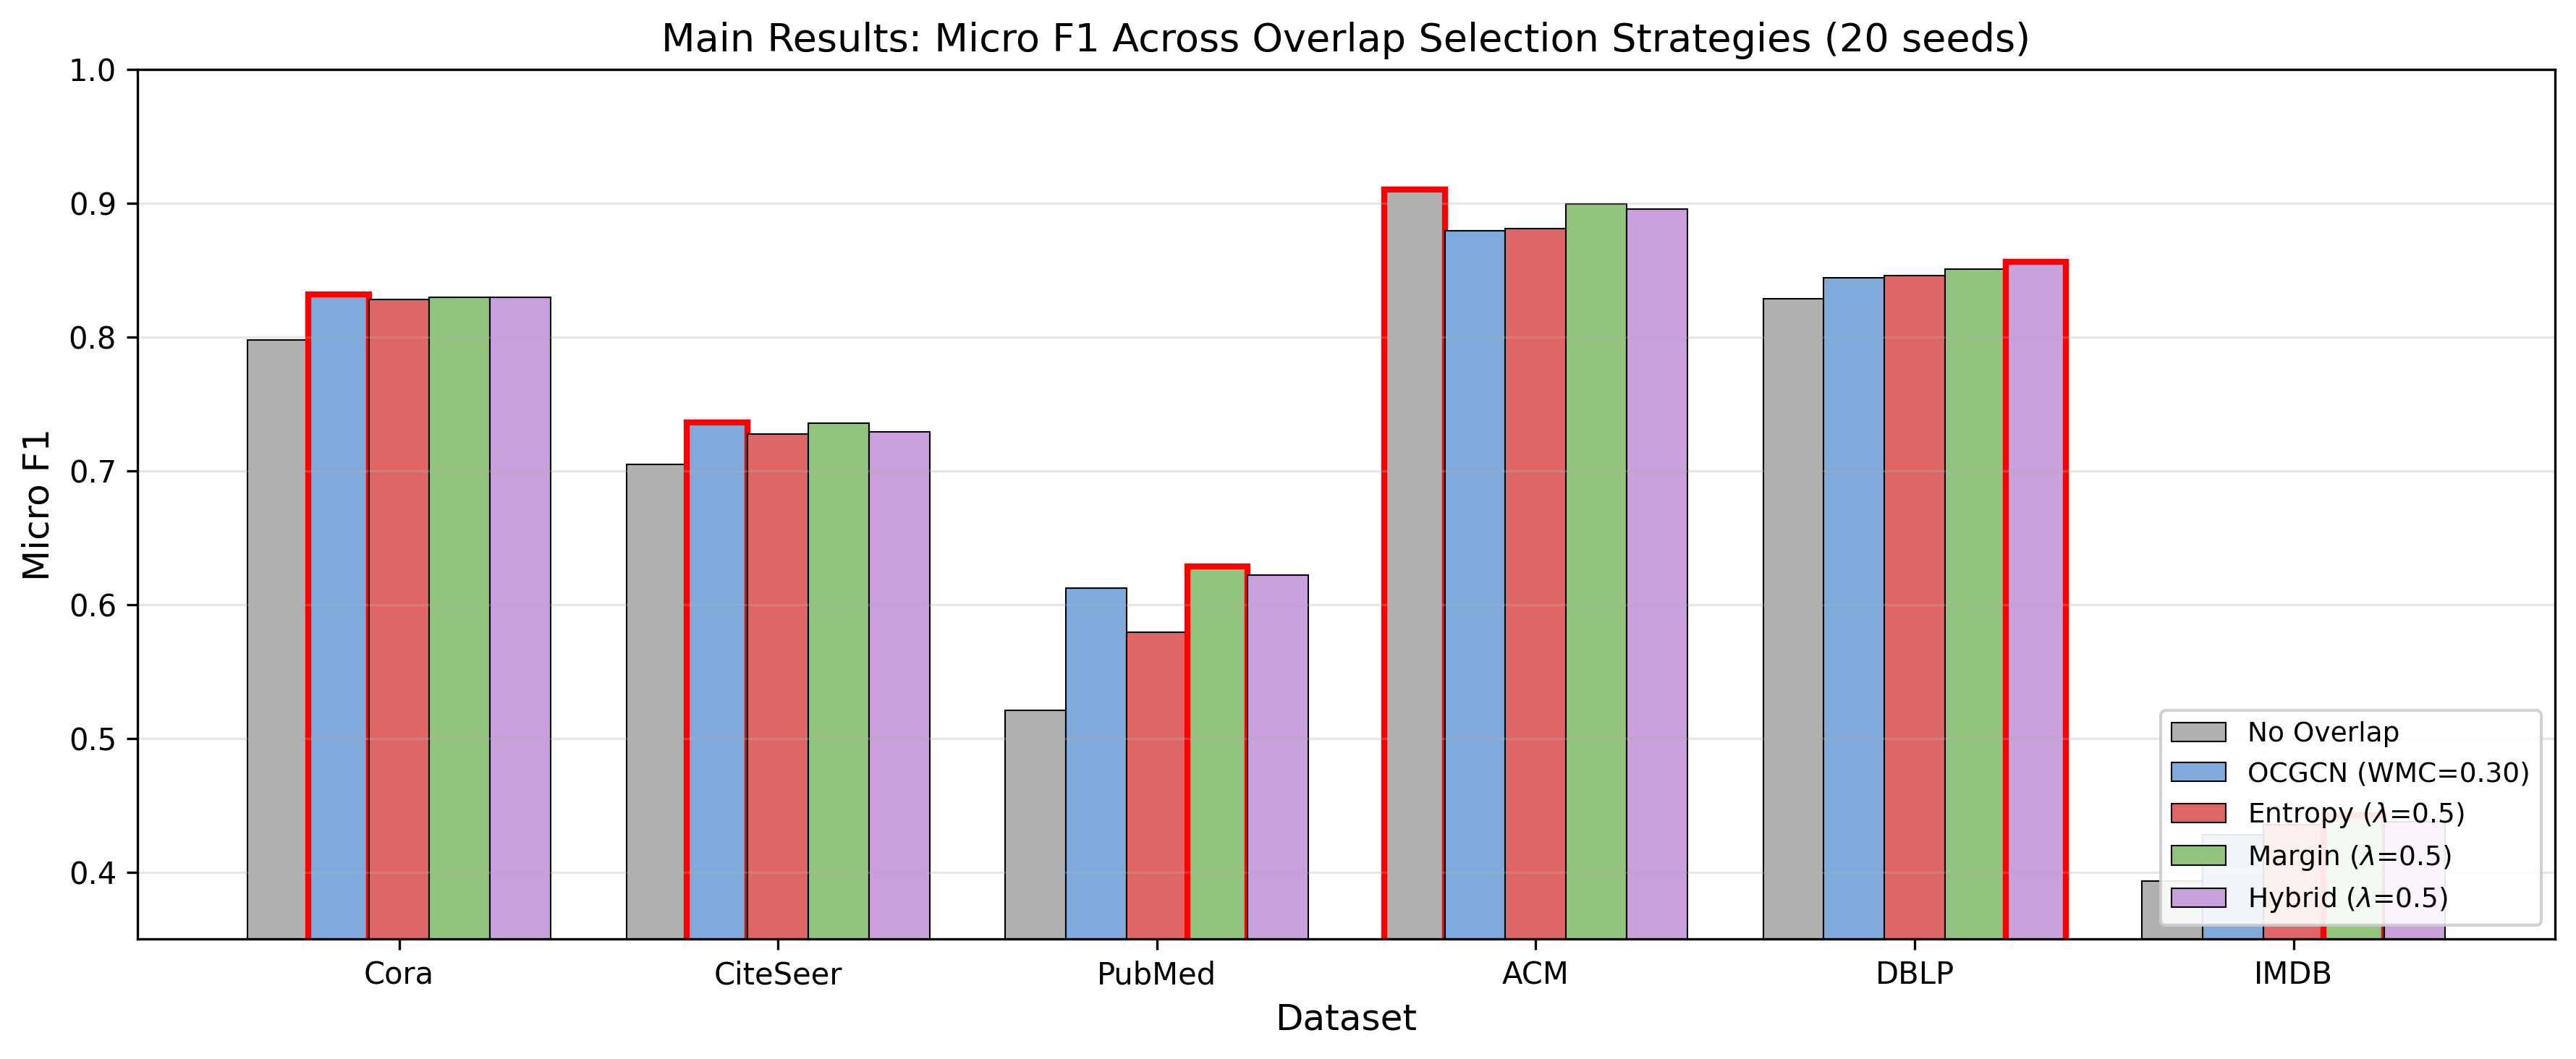
\includegraphics[width=\textwidth]{figures/main_results_comparison.png}
\caption{Micro F1 scores across all overlap selection strategies (20 seeds). Bars with red outlines indicate the best result per dataset. Adaptive methods are competitive with or outperform the fixed WMC default on most datasets; on ACM the no-overlap configuration is best.}
\label{fig:main-results}
\end{figure}

\subsubsection{Ablation: Adaptation Strength}
\label{subsec:ablation}

Tables~\ref{tab:entropy-lambda},~\ref{tab:margin-lambda} and~\ref{tab:hybrid-lambda} examine the effect of $\lambda$ on the three adaptive strategies.

\begin{table}[ht]
\centering
\caption{Entropy-Adaptive Micro F1 for different $\lambda$ values (10 seeds). Optimal $\lambda$ per dataset in bold.}
\label{tab:entropy-lambda}
\begin{tabular}{lcccc}
\toprule
\textbf{Dataset} & $\lambda$=0.25 & $\lambda$=0.50 & $\lambda$=0.75 & \textbf{Optimal} \\
\midrule
Cora      & 0.823 & 0.822 & \textbf{0.831} & 0.75 \\
CiteSeer  & 0.735 & \textbf{0.740} & 0.739 & 0.50 \\
PubMed    & 0.591 & \textbf{0.601} & 0.582 & 0.50 \\
ACM       & 0.864 & 0.888 & \textbf{0.902} & 0.75 \\
DBLP      & 0.850 & 0.843 & \textbf{0.853} & 0.75 \\
IMDB      & 0.433 & 0.440 & \textbf{0.442} & 0.75 \\
\bottomrule
\end{tabular}
\end{table}

\begin{table}[ht]
\centering
\caption{Margin-Adaptive Micro F1 for different $\lambda$ values (10 seeds). Optimal $\lambda$ per dataset in bold.}
\label{tab:margin-lambda}
\begin{tabular}{lcccc}
\toprule
\textbf{Dataset} & $\lambda$=0.25 & $\lambda$=0.50 & $\lambda$=0.75 & \textbf{Optimal} \\
\midrule
Cora      & 0.817 & 0.820 & \textbf{0.825} & 0.75 \\
CiteSeer  & 0.722 & \textbf{0.745} & 0.738 & 0.50 \\
PubMed    & 0.604 & 0.612 & \textbf{0.645} & 0.75 \\
ACM       & 0.847 & \textbf{0.907} & 0.880 & 0.50 \\
DBLP      & \textbf{0.857} & 0.851 & 0.852 & 0.25 \\
IMDB      & 0.436 & 0.441 & \textbf{0.447} & 0.75 \\
\bottomrule
\end{tabular}
\end{table}

\begin{table}[ht]
\centering
\caption{Hybrid-Adaptive Micro F1 for different $\lambda$ values (10 seeds). Optimal $\lambda$ per dataset in bold.}
\label{tab:hybrid-lambda}
\begin{tabular}{lcccc}
\toprule
\textbf{Dataset} & $\lambda$=0.25 & $\lambda$=0.50 & $\lambda$=0.75 & \textbf{Optimal} \\
\midrule
Cora      & 0.818 & \textbf{0.825} & 0.812 & 0.50 \\
CiteSeer  & 0.741 & \textbf{0.742} & 0.738 & 0.50 \\
PubMed    & 0.616 & 0.602 & \textbf{0.628} & 0.75 \\
ACM       & 0.885 & \textbf{0.910} & 0.870 & 0.50 \\
DBLP      & 0.857 & \textbf{0.863} & 0.853 & 0.50 \\
IMDB      & 0.433 & 0.436 & \textbf{0.448} & 0.75 \\
\bottomrule
\end{tabular}
\end{table}

IMDB, which has the highest mean entropy (0.419) and highest overlap ratio (0.621), benefits from stronger adaptation at $\lambda = 0.75$ across all variants.
Margin-Adaptive shows the most per-dataset variation: DBLP prefers the lightest adaptation ($\lambda = 0.25$), while PubMed and IMDB prefer $\lambda = 0.75$.
Figures~\ref{fig:entropy-lambda},~\ref{fig:margin-lambda} and~\ref{fig:hybrid-lambda} visualize the lambda sensitivity.

\begin{figure}[ht]
\centering
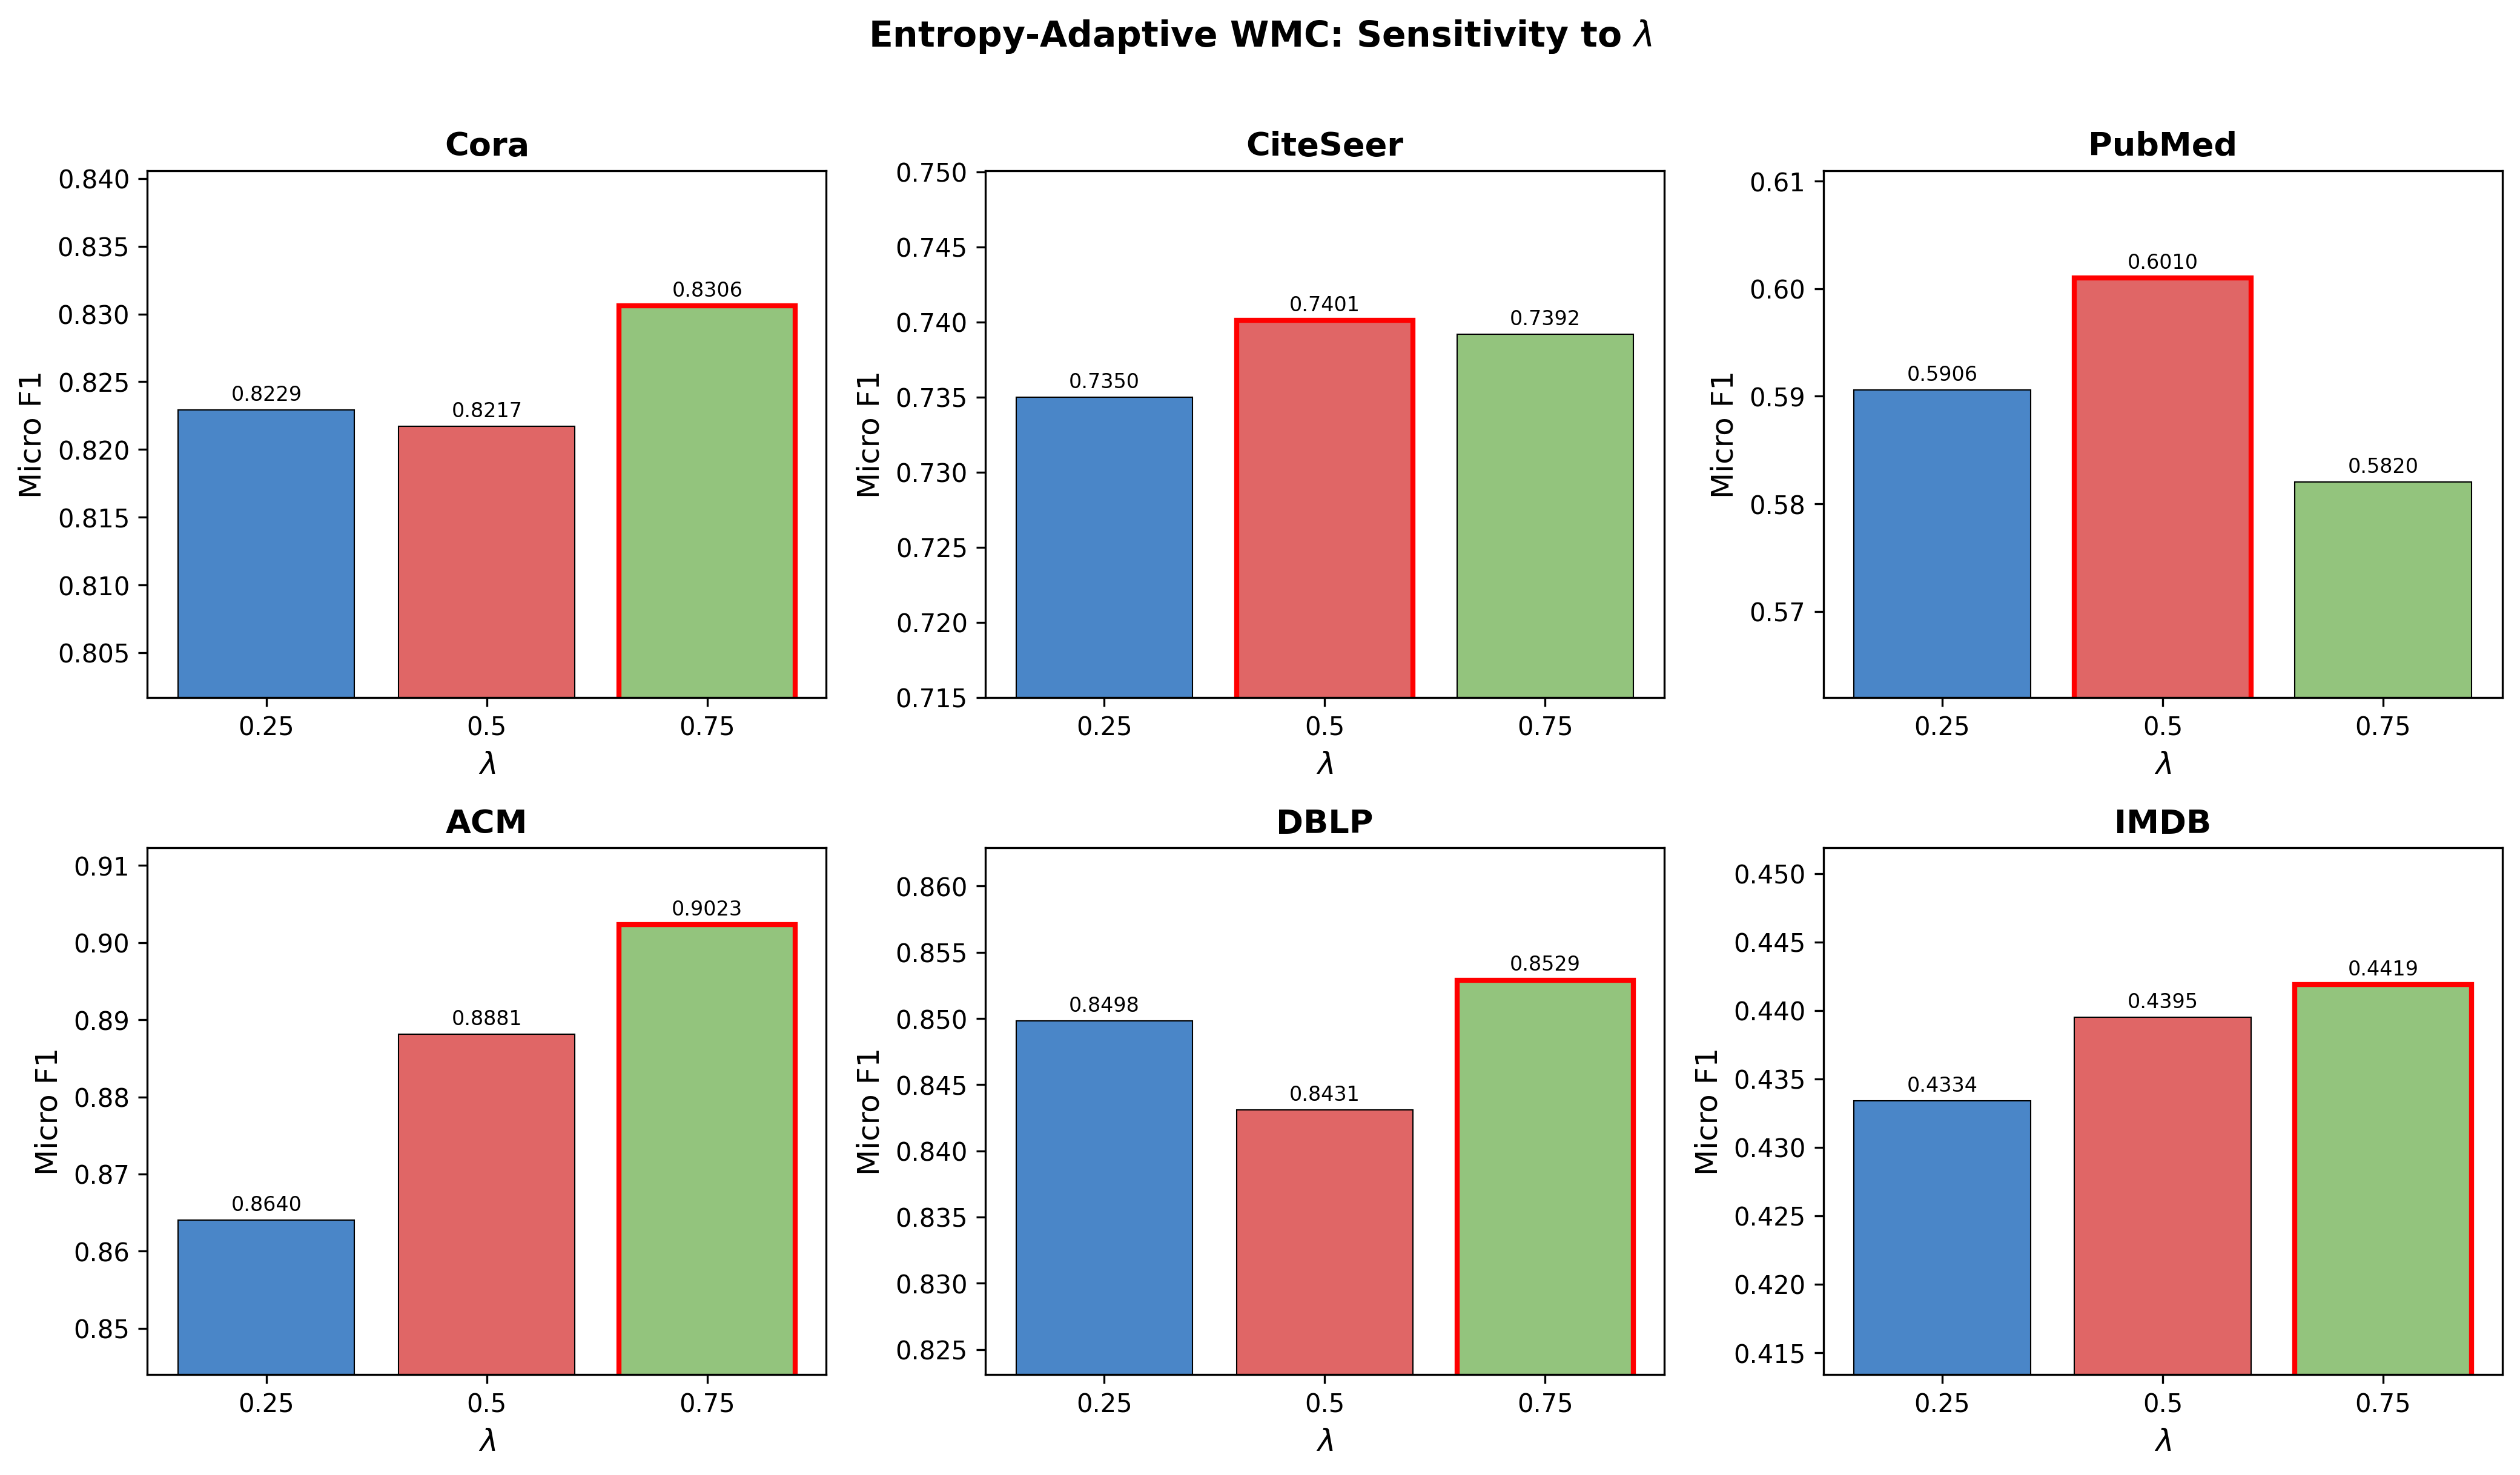
\includegraphics[width=\textwidth]{figures/entropy_lambda_sensitivity.png}
\caption{Entropy-Adaptive WMC performance as a function of $\lambda$ for each dataset. Red-bordered bars indicate the optimal $\lambda$. $\lambda = 0.75$ is optimal for four of six datasets.}
\label{fig:entropy-lambda}
\end{figure}

\begin{figure}[ht]
\centering
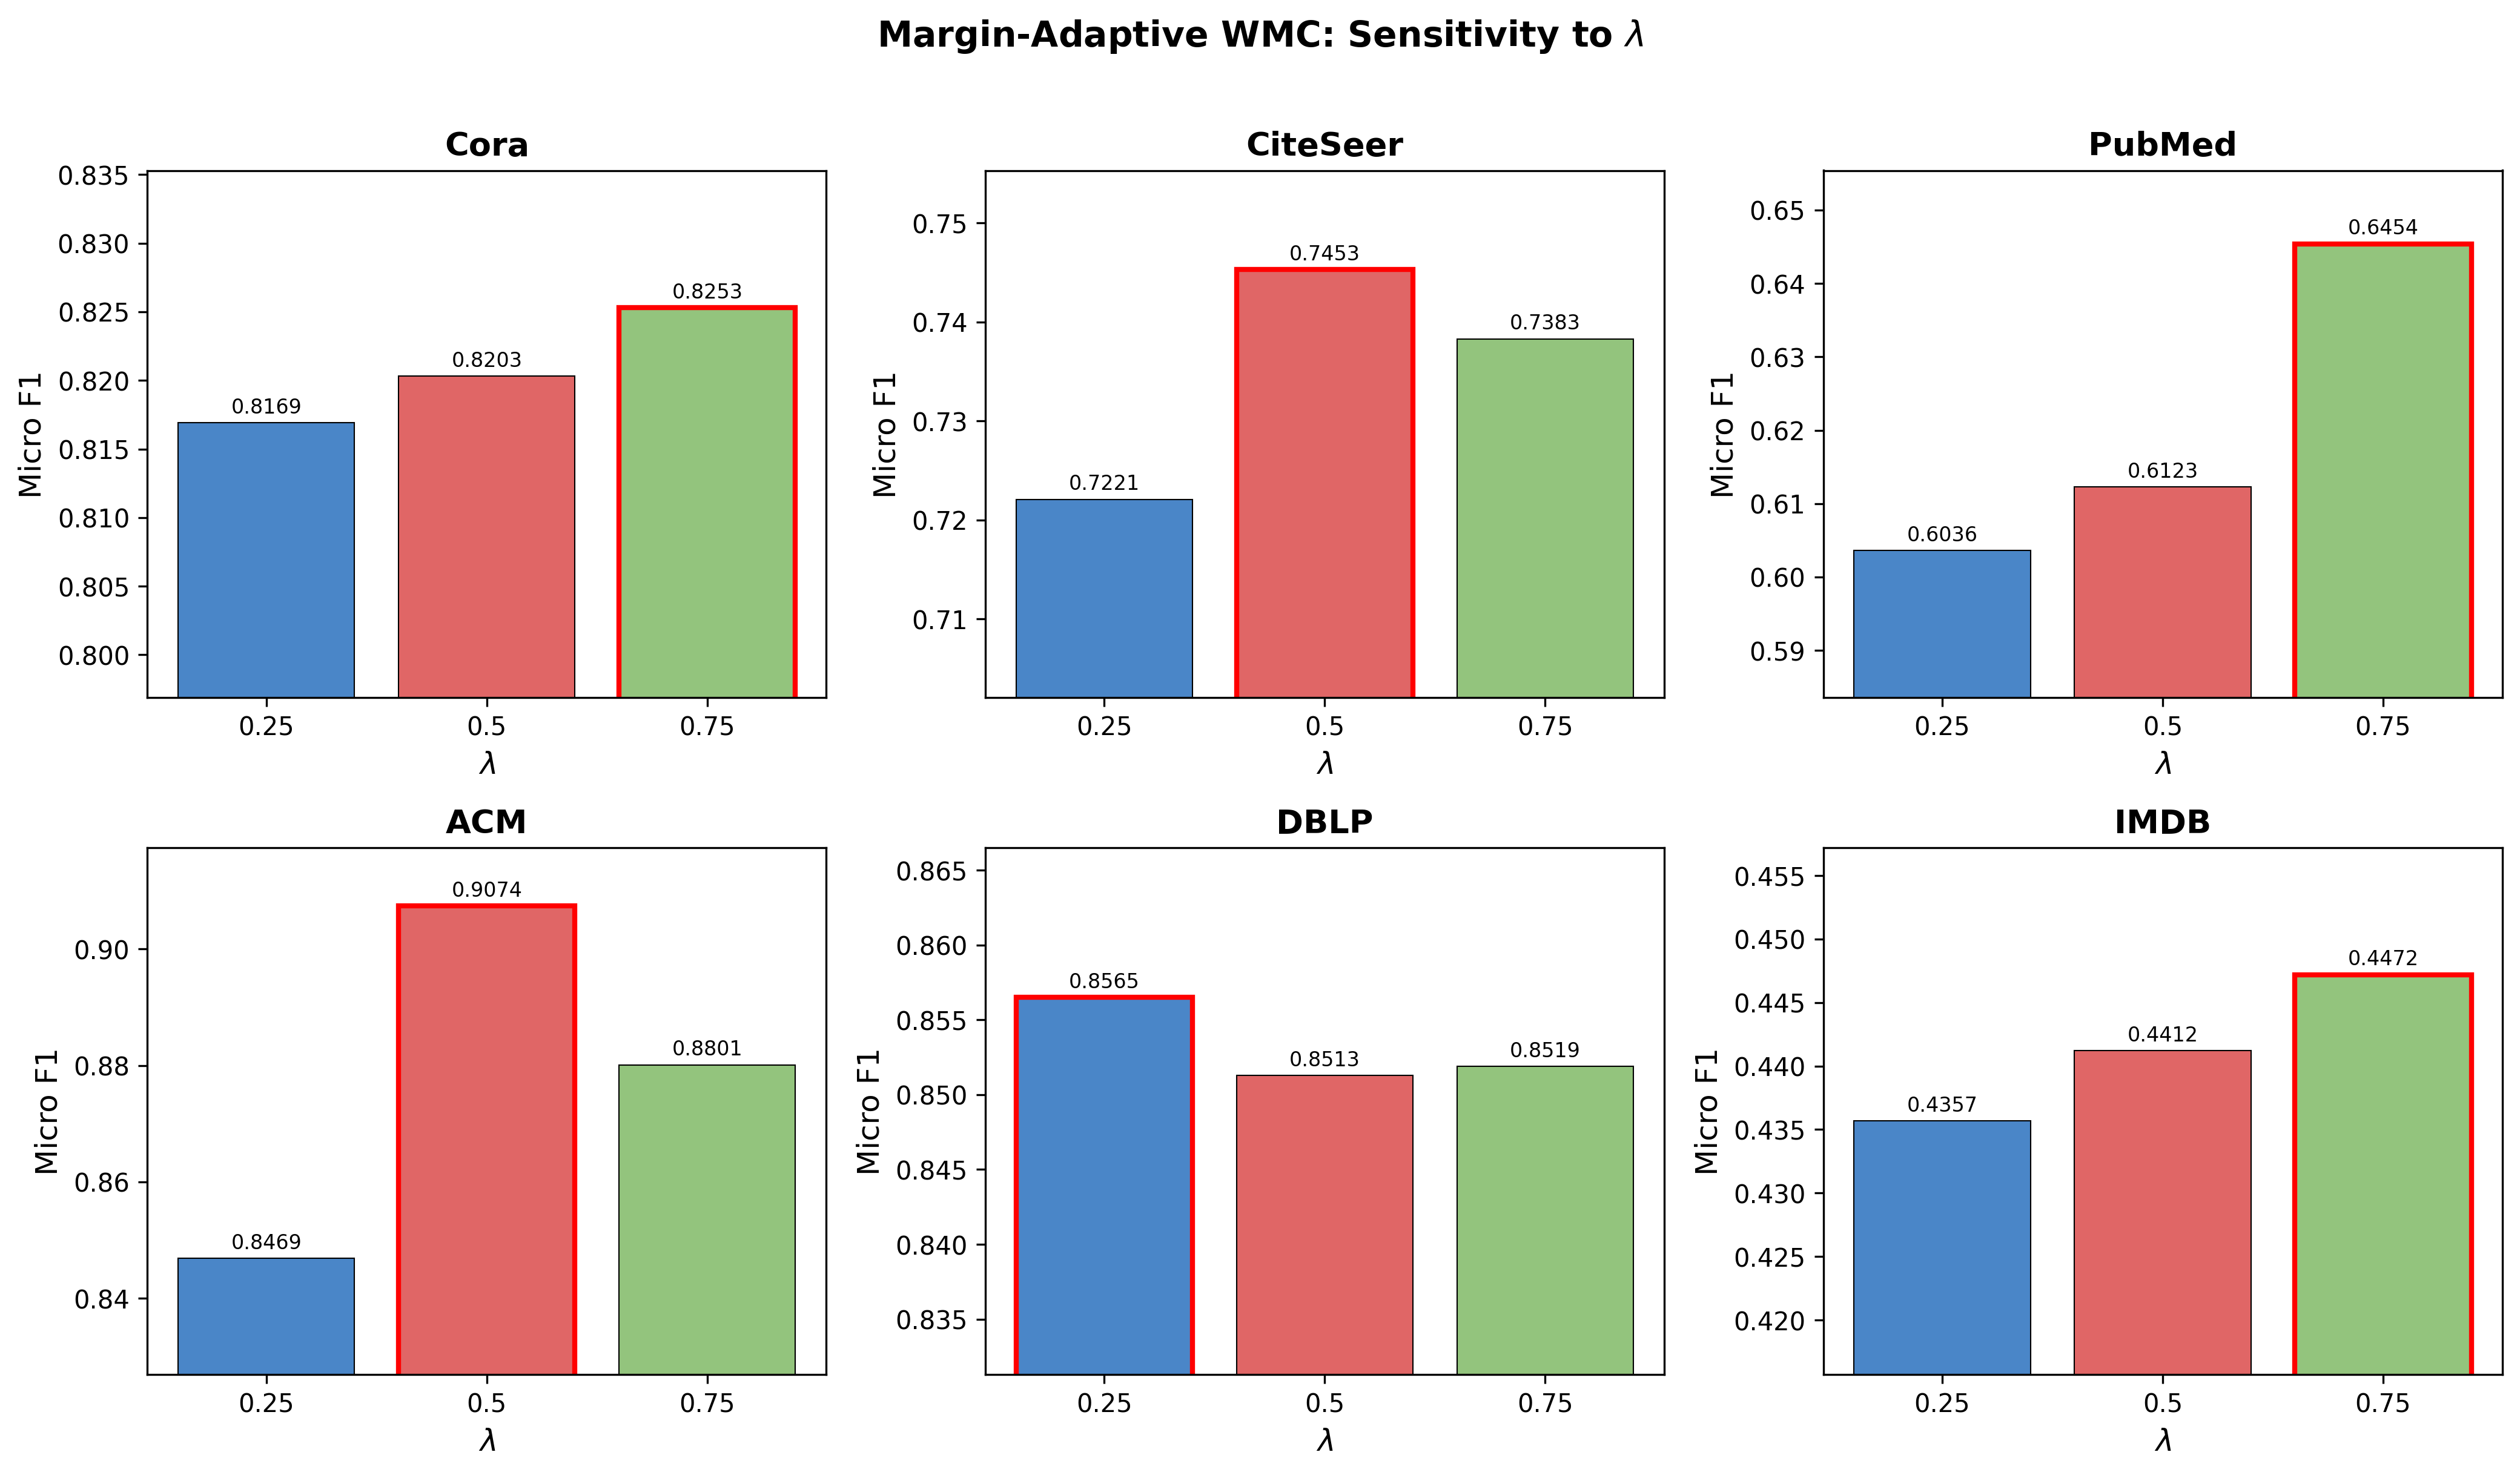
\includegraphics[width=\textwidth]{figures/margin_lambda_sensitivity.png}
\caption{Margin-Adaptive WMC performance as a function of $\lambda$ for each dataset. Red-bordered bars indicate the optimal $\lambda$. Margin-Adaptive shows the most per-dataset variation.}
\label{fig:margin-lambda}
\end{figure}

\begin{figure}[ht]
\centering
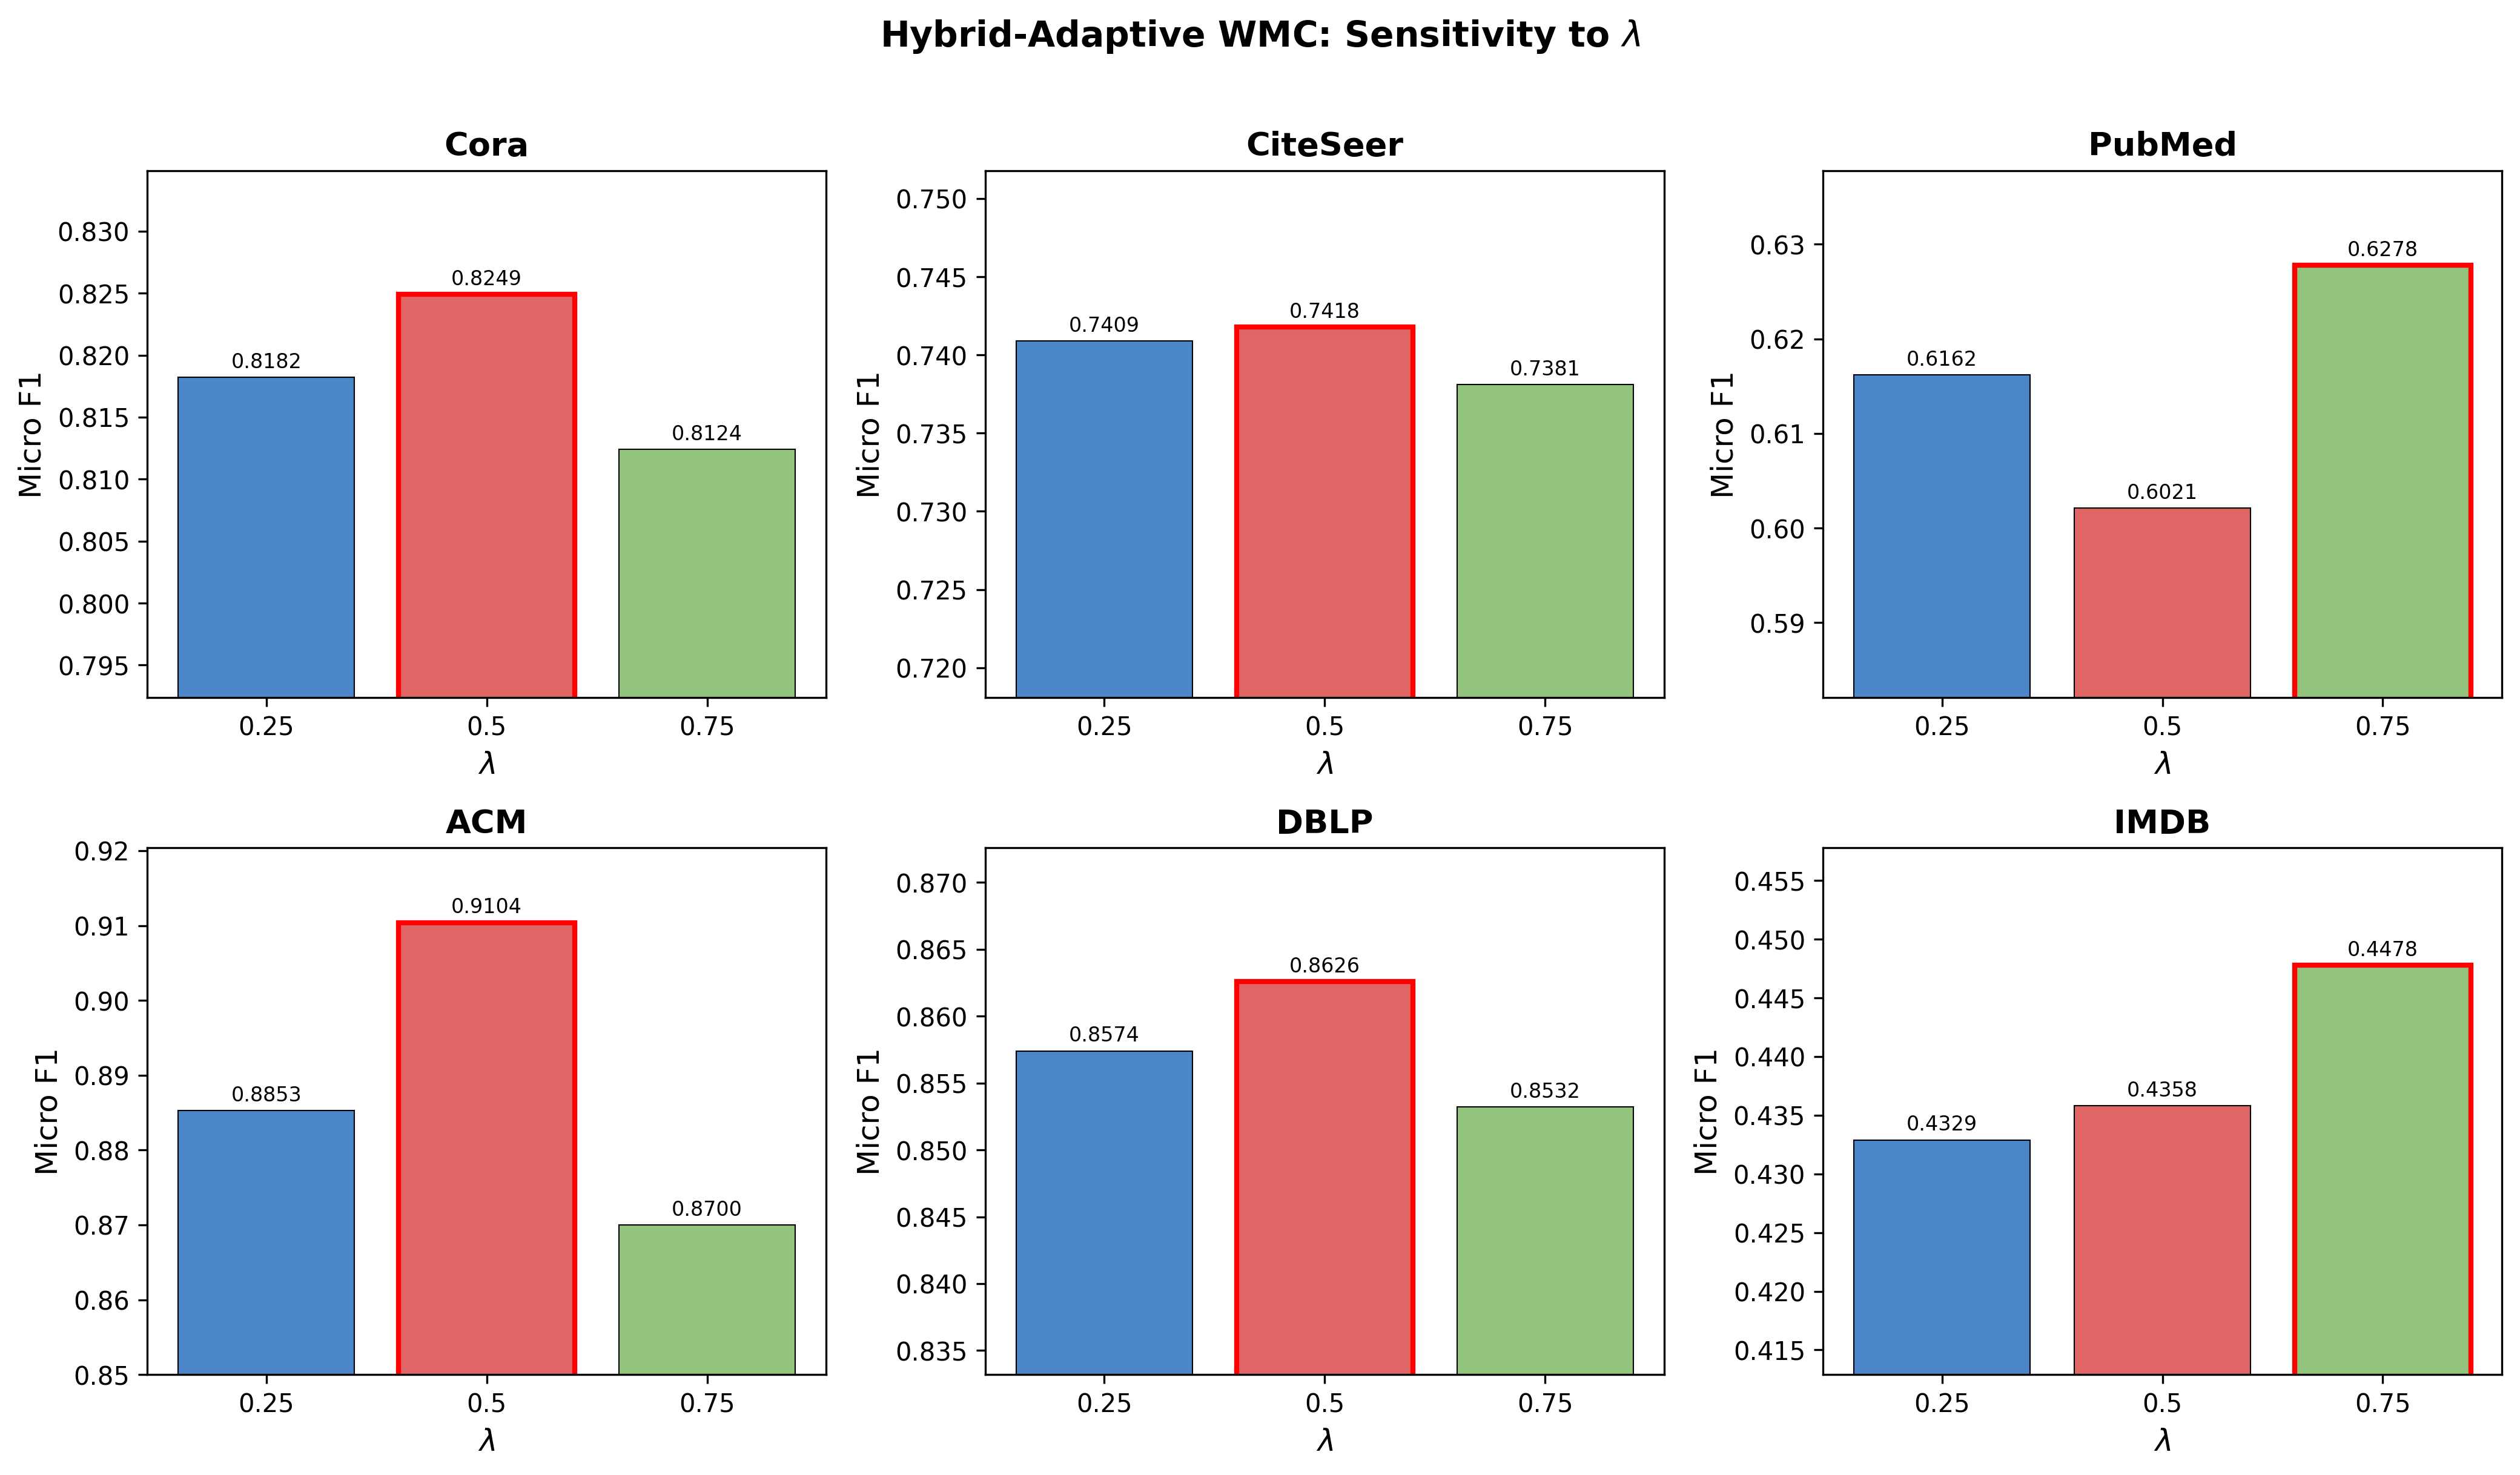
\includegraphics[width=\textwidth]{figures/hybrid_lambda_sensitivity.png}
\caption{Hybrid-Adaptive WMC performance as a function of $\lambda$ for each dataset. Red-bordered bars indicate the optimal $\lambda$. $\lambda = 0.50$ is optimal for four of six datasets, making the hybrid the most stable configuration.}
\label{fig:hybrid-lambda}
\end{figure}

\clearpage

\subsubsection{Fair Comparison: Equal Overlap Ratios}
\label{subsec:fair-comparison}

A critical question is whether adaptive methods perform better because they select better overlap nodes, or simply because they generate more overlap.
Table~\ref{tab:fair-comparison} compares adaptive methods against the closest fixed-WMC baseline at matched overlap ratios.

\begin{table}[ht]
\centering
\caption{Fair comparison at matched overlap ratios.}
\label{tab:fair-comparison}
\begin{tabular}{llcccll}
\toprule
\textbf{Dataset} & \textbf{Adaptive} & \textbf{Overlap} & \textbf{Closest Fixed} & \textbf{Overlap} & \textbf{$\Delta$F1} & \textbf{Winner} \\
\midrule
Cora    & margin & 1.44 & WMC=0.20 & 1.48 & +0.005 & Adaptive \\
DBLP    & hybrid & 1.33 & WMC=0.20 & 1.35 & +0.013 & Adaptive \\
PubMed  & margin & 1.31 & WMC=0.20 & 1.35 & $-$0.032 & Fixed \\
ACM     & margin & 1.31 & WMC=0.20 & 1.35 & +0.018 & Adaptive \\
CiteSeer & margin & 1.18 & WMC=0.30 & 1.15 & +0.000 & Tie \\
IMDB    & margin & 2.53 & WMC=0.20 & 2.56 & +0.003 & Adaptive \\
\bottomrule
\end{tabular}
\end{table}

At equal overlap ratios, adaptive methods win on four of six datasets (CiteSeer is a statistical tie, $\Delta$F1 = +0.000; PubMed is the only loss at $-$0.032), with gains ranging from +0.003 (IMDB) to +0.018 (ACM).
Fixed WMC wins only on PubMed ($-$0.032), where adaptive methods underperform at matched overlap.
This indicates that adaptive selection identifies higher-quality overlap nodes in most cases.
Figure~\ref{fig:fair-comparison} visualizes this comparison.

\begin{figure}[ht]
\centering
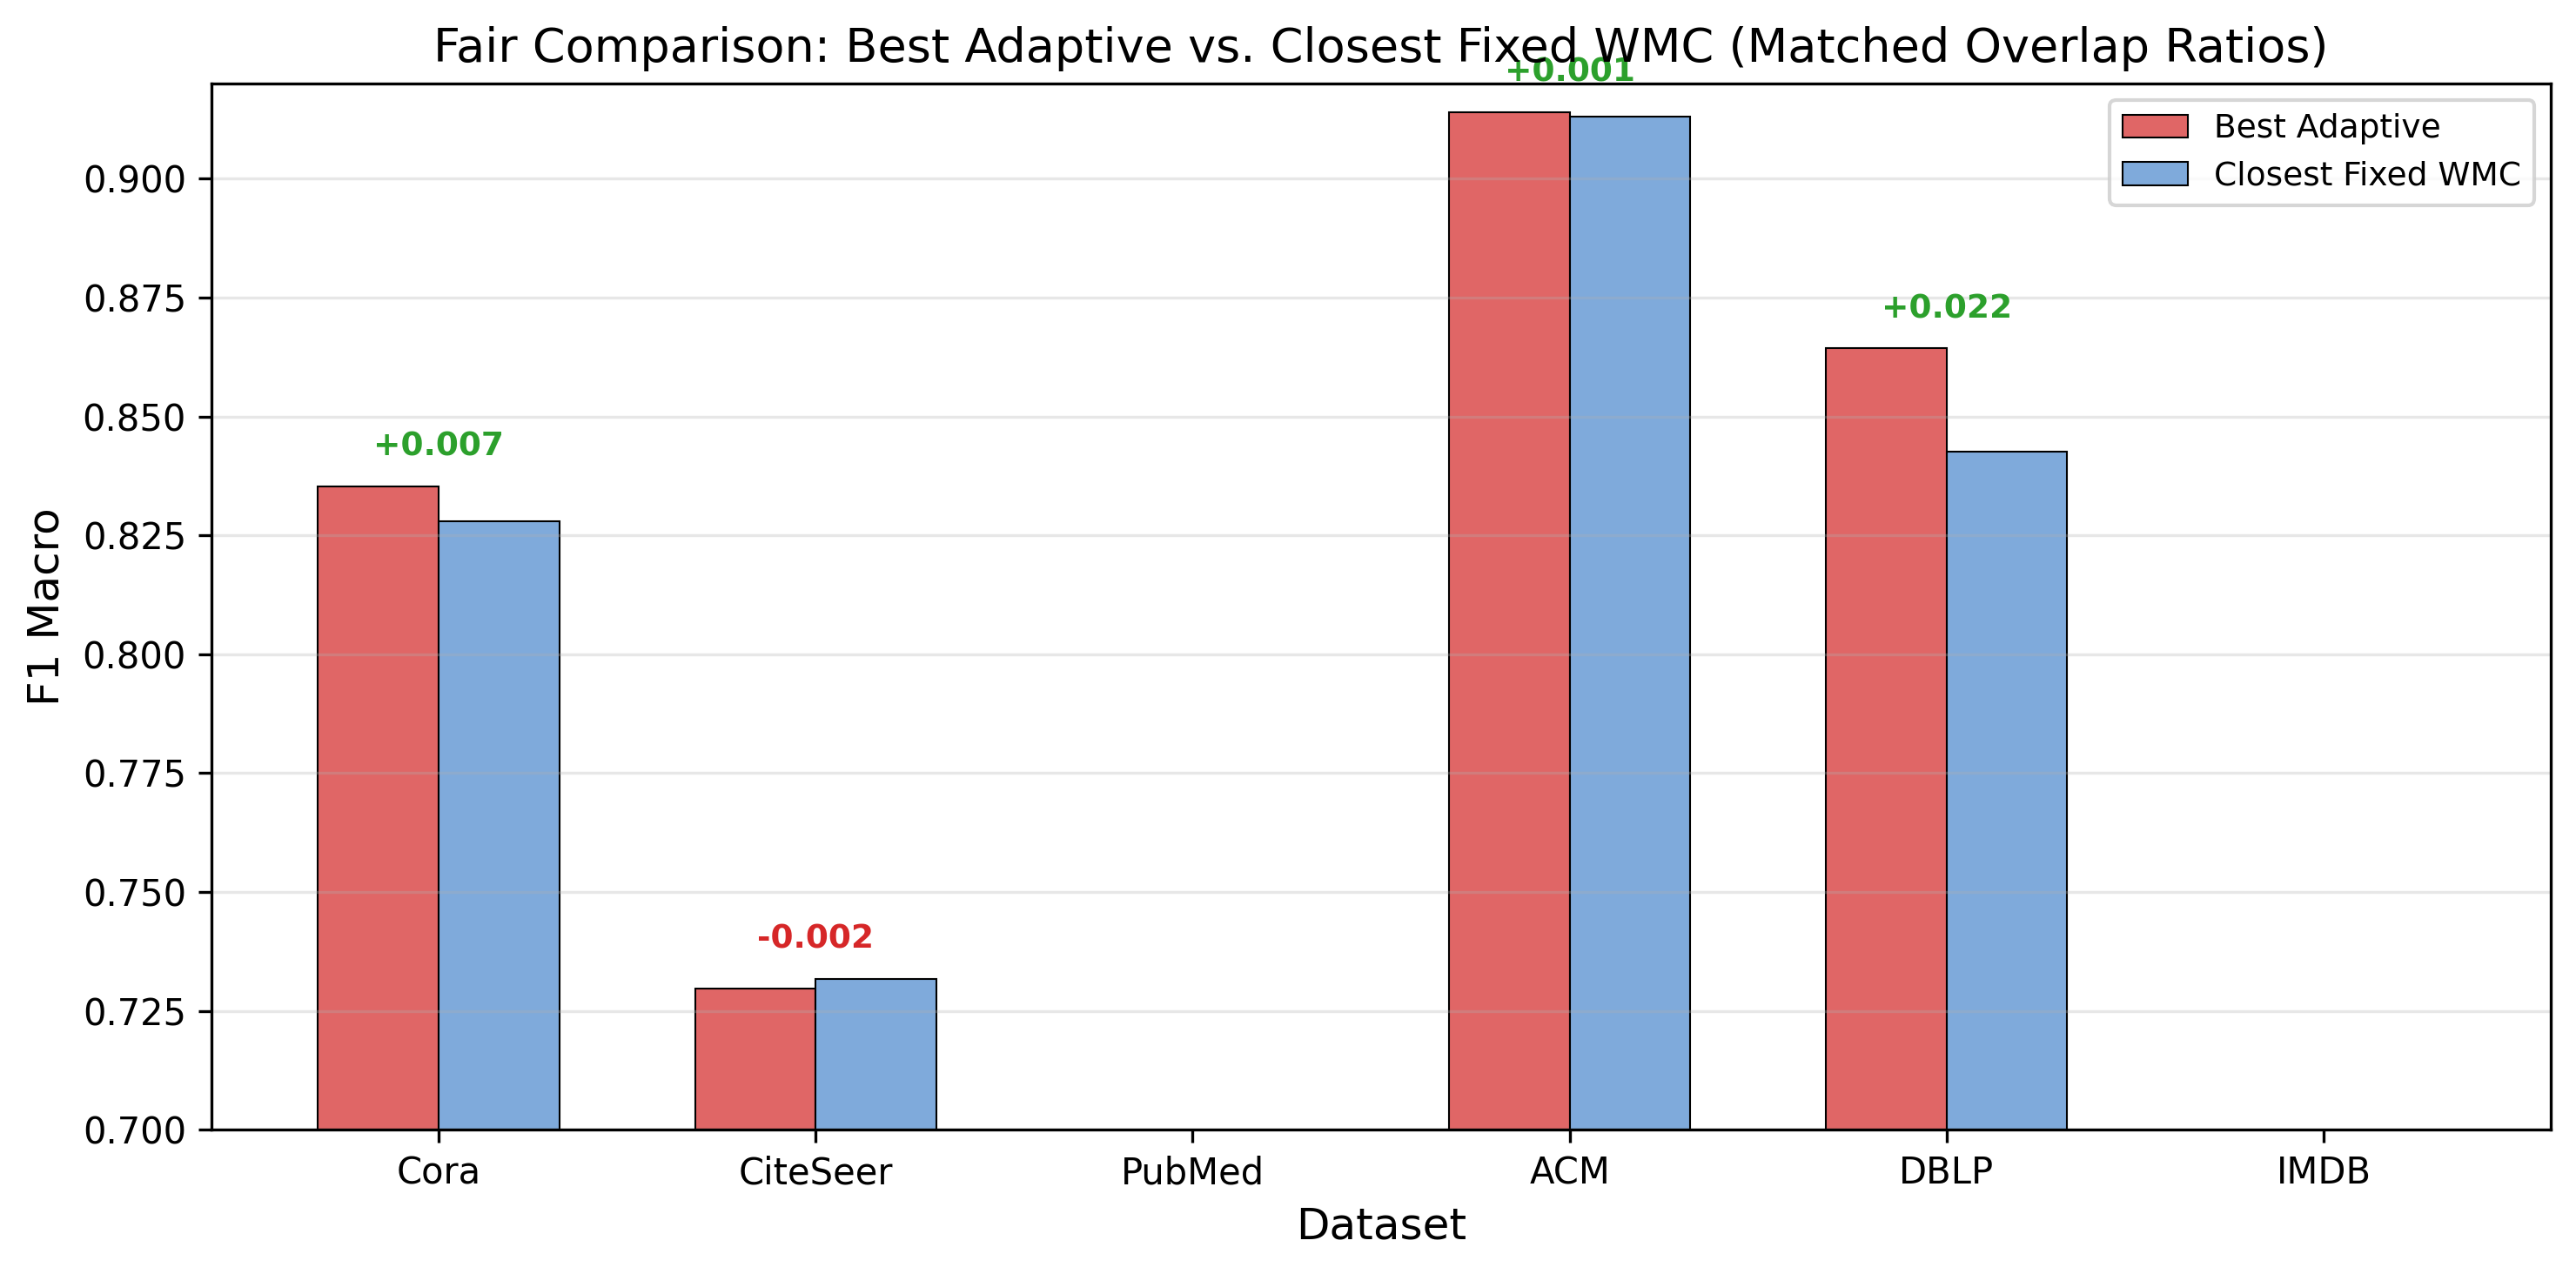
\includegraphics[width=\textwidth]{figures/fair_comparison.png}
\caption{Fair comparison at matched overlap ratios (micro F1). Green annotations indicate adaptive wins; red indicates fixed wins. Adaptive methods win on four of six datasets (CiteSeer is a statistical tie and PubMed the only loss), with the largest gain on ACM (+0.018).}
\label{fig:fair-comparison}
\end{figure}

\subsubsection{Overlap Efficiency}
\label{subsec:efficiency}

	
We define overlap efficiency as the F1 gain per unit overlap increase relative to the no-overlap baseline.
Table~\ref{tab:efficiency} presents this metric for each method.

\begin{table}[ht]
\centering
\caption{Overlap efficiency (F1 gain / overlap ratio increase) for each method.}
\label{tab:efficiency}
\begin{tabular}{lcccccc}
\toprule
\textbf{Method} & \textbf{Cora} & \textbf{DBLP} & \textbf{PubMed} & \textbf{ACM} & \textbf{CiteSeer} & \textbf{IMDB} \\
\midrule
WMC=0.10           & 0.049 & 0.056 & 0.252 & $-$0.043 & 0.092 & 0.026 \\
WMC=0.20           & 0.056 & 0.042 & 0.402 & $-$0.084 & 0.122 & 0.030 \\
WMC=0.30           & 0.092 & 0.063 & 0.342 & $-$0.118 & 0.204 & 0.029 \\
\textbf{Entropy}   & 0.073 & 0.054 & 0.190 & $-$0.096 & 0.128 & 0.027 \\
\textbf{Margin}    & 0.073 & 0.066 & 0.341 & $-$0.036 & 0.169 & 0.032 \\
\textbf{Hybrid}    & 0.072 & 0.083 & 0.317 & $-$0.047 & 0.129 & 0.028 \\
\bottomrule
\end{tabular}
\end{table}

Among the fixed thresholds shown, WMC~=~0.30 achieves the highest efficiency on Cora (0.092) and CiteSeer (0.204), while WMC~=~0.20 is most efficient on PubMed (0.402).
Among adaptive methods, Margin-Adaptive is the most efficient on PubMed (0.341) and IMDB (0.032), Hybrid-Adaptive on DBLP (0.083), and Entropy-Adaptive on Cora (0.073, tied with Margin).
Efficiency is negative for every method on ACM, consistent with overlap providing no benefit on that dataset.
Averaged across all six datasets, Margin-Adaptive achieves the highest mean efficiency (0.108),
edging out the best fixed threshold WMC~=~0.30 (0.102), which indicates that adaptive methods
extract slightly more F1 gain per unit of overlap added.
Figure~\ref{fig:efficiency} visualizes overlap efficiency across methods.

\begin{figure}[ht]
\centering
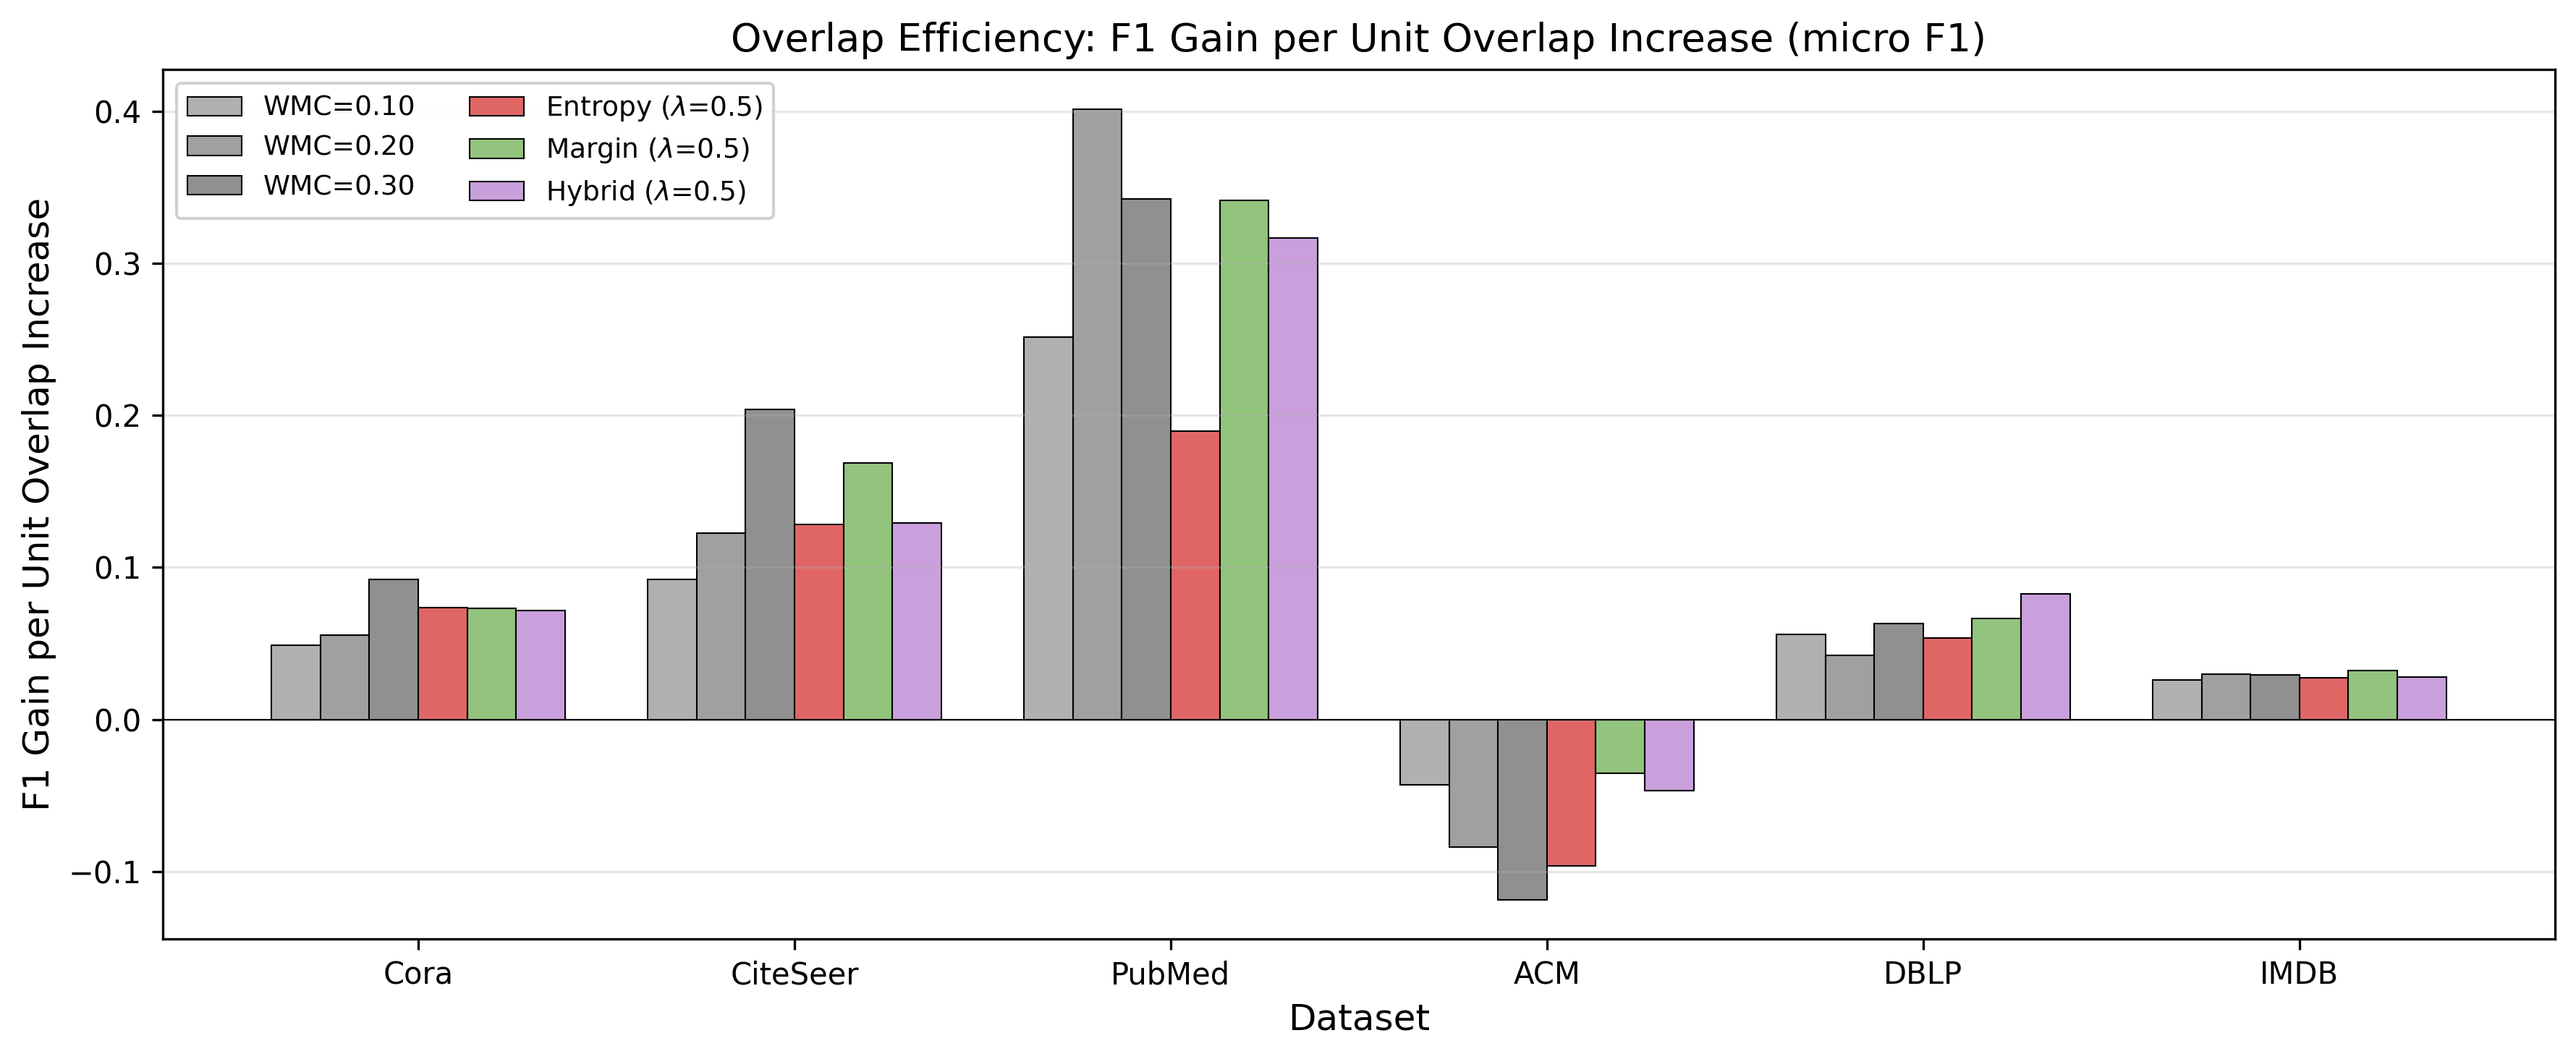
\includegraphics[width=\textwidth]{figures/overlap_efficiency.png}
\caption{Overlap efficiency (F1 gain per unit overlap increase, micro F1) for each method. Adaptive methods match fixed thresholds in efficiency on most datasets; Margin-Adaptive is the most efficient adaptive variant on PubMed and IMDB.}
\label{fig:efficiency}
\end{figure}

\subsubsection{Training Time and Computational Overhead}
\label{subsec:runtime}

Table~\ref{tab:runtime} reports the measured wall-clock training time per run (mean over 20 seeds) for the main configurations, together with the one-time DANMF decomposition cost. The adaptive selection itself adds negligible overhead: entropy and margin scores are computed once per node in $O(K)$ and $O(K \log K)$, adding at most a few milliseconds to the pipeline. Training time is dominated by the GCN epochs and grows with the size of the cluster subgraphs; because adaptive methods produce slightly larger subgraphs (more overlap nodes), their per-run time is marginally higher than the no-overlap configuration (e.g., Cora: 1.59\,s no-overlap vs.\ 1.62\,s margin-adaptive), but remains well below the one-time DANMF cost on the larger graphs.

\begin{table}[ht]
\centering
\caption{Training time (seconds, mean over 20 seeds; DANMF fit is a single one-time measurement) on an NVIDIA RTX 3090.}
\label{tab:runtime}
\begin{tabular}{lrrrrrr}
\toprule
\textbf{Dataset} & \textbf{DANMF fit} & \textbf{No overlap} & \textbf{WMC=0.30} & \textbf{Margin} & \textbf{Hybrid} & \textbf{Entropy} \\
\midrule
Cora      & 2.5  & 1.59 & 1.60 & 1.62 & 1.68 & 1.63 \\
CiteSeer  & 2.5  & 1.56 & 1.61 & 1.67 & 1.72 & 1.67 \\
PubMed    & 36.1  & 1.41 & 1.87 & 2.00 & 2.33 & 2.19 \\
ACM       & 2.4  & 0.80 & 0.91 & 0.86 & 1.04 & 0.97 \\
DBLP      & 1.7  & 1.05 & 0.98 & 1.01 & 1.13 & 1.09 \\
IMDB      & 22.1  & 1.62 & 2.42 & 2.53 & 2.52 & 2.48 \\
\bottomrule
\end{tabular}
\end{table}

Figure~\ref{fig:runtime} visualizes the per-run training time and the one-time decomposition cost.

\begin{figure}[ht]
\centering
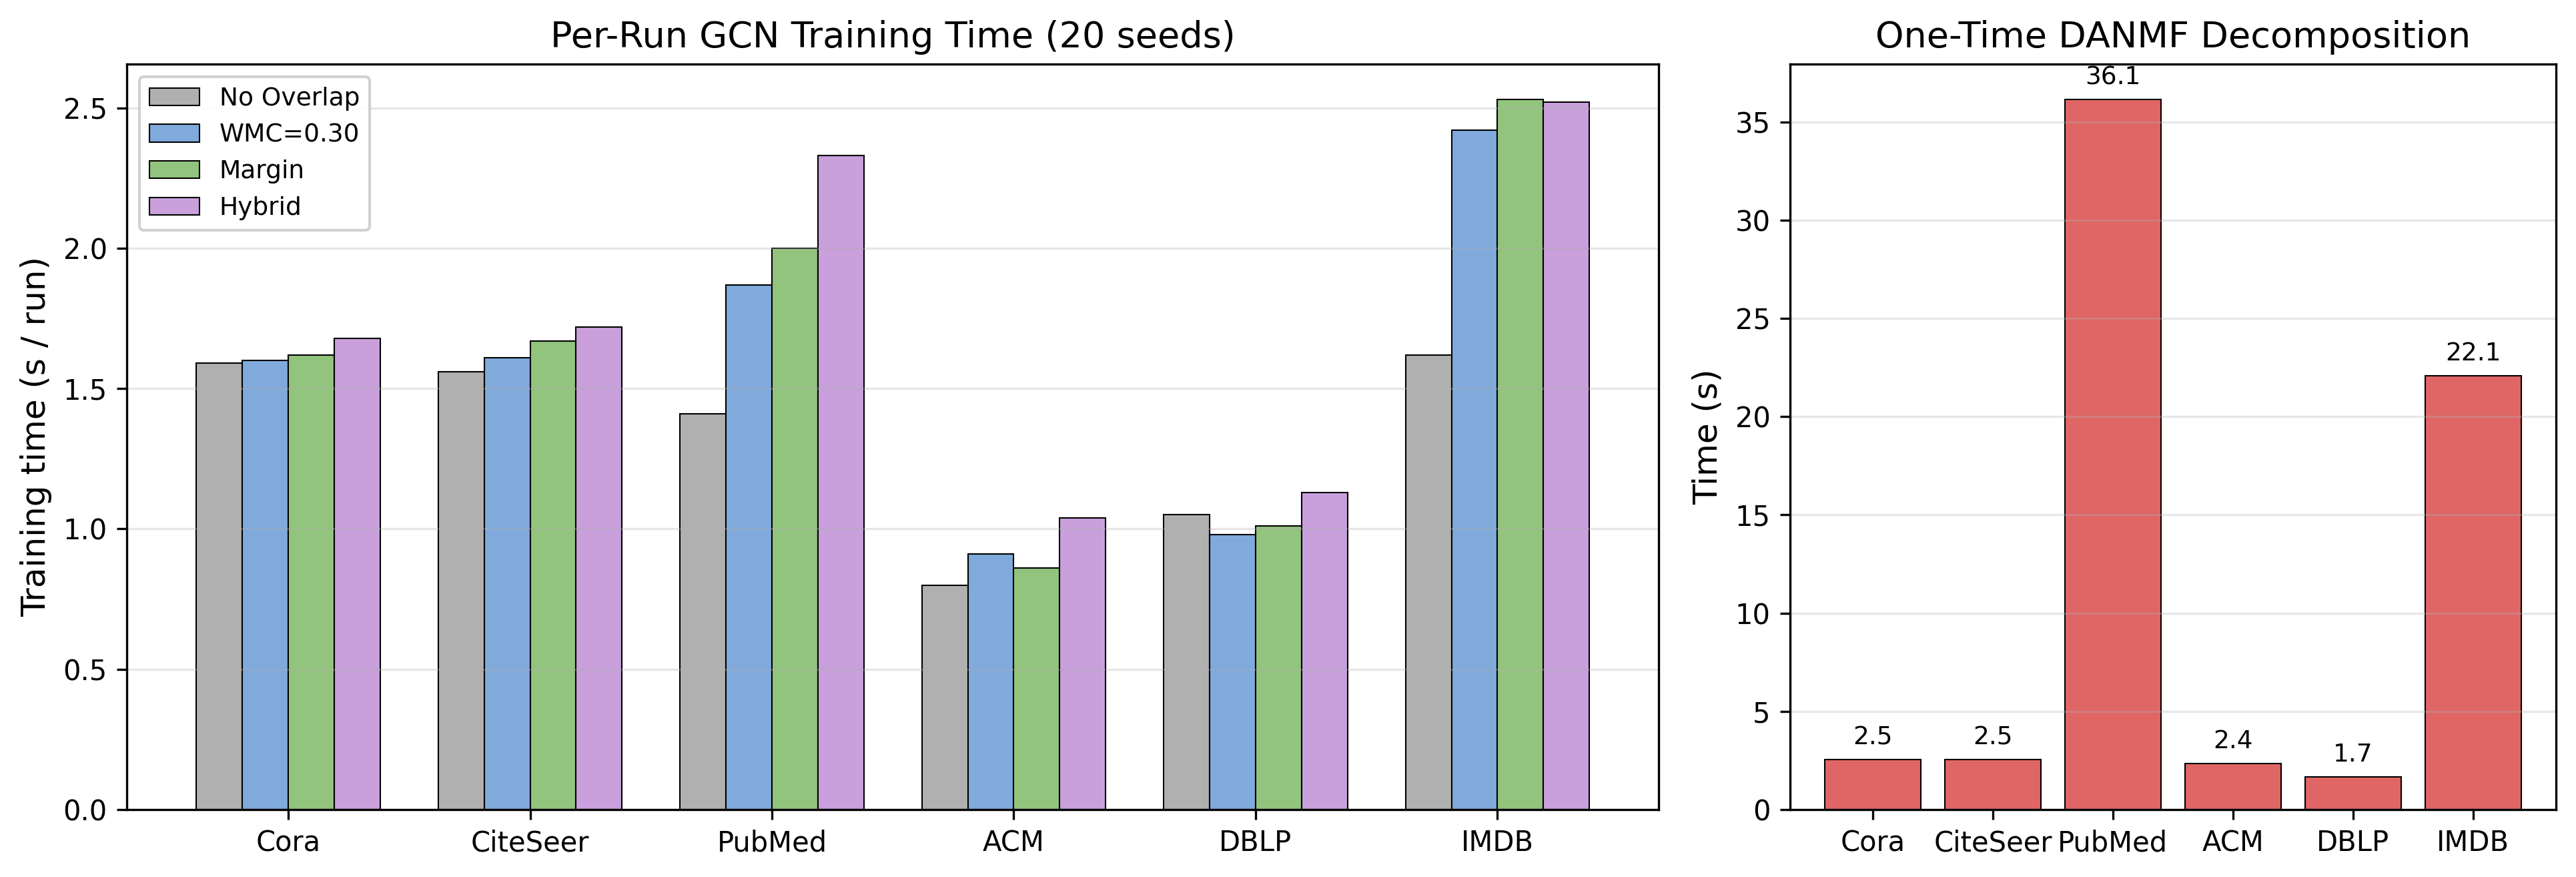
\includegraphics[width=\textwidth]{figures/runtime_comparison.png}
\caption{Left: mean GCN training time per run (20 seeds) for no-overlap, WMC=0.30, margin-adaptive, and hybrid-adaptive. Right: one-time DANMF decomposition cost per dataset. Training time is dominated by the GCN and grows with subgraph size; the adaptive selection itself adds negligible overhead.}
\label{fig:runtime}
\end{figure}

%%======================================================================
\subsubsection{Statistical Significance}
\label{subsec:significance}

Paired $t$-tests and Wilcoxon signed-rank tests comparing adaptive methods against the untuned default WMC~=~0.30 (20 seeds each), together with pooled tests across all 120 paired runs, are reported in Table~\ref{tab:stats}.

\begin{table}[ht]
\centering
\caption{Paired statistical tests (micro F1, 20 seeds): best adaptive method vs.\ the untuned default WMC~=~0.30, plus pooled tests across all 120 paired runs.}
\label{tab:stats}
\begin{tabular}{llllccc}
\toprule
\textbf{Setting} & \textbf{Adaptive} & \textbf{vs} & \textbf{$t$-stat} & \textbf{$p$-val} & \textbf{Wilcoxon $p$} & \textbf{Winner} \\
\midrule
DBLP      & hybrid & WMC=0.30 & 2.538 & 0.020 & 0.036 & Adaptive \\
IMDB      & margin & WMC=0.30 & 3.402 & 0.003 & 0.003 & Adaptive \\
IMDB      & hybrid & WMC=0.30 & 2.285 & 0.034 & 0.048 & Adaptive \\
PubMed    & margin & WMC=0.30 & 1.025 & 0.318 & 0.452 & No diff \\
ACM       & margin & WMC=0.30 & 1.428 & 0.169 & 0.189 & No diff \\
Cora      & margin & WMC=0.30 & $-$0.347 & 0.733 & 0.784 & No diff \\
CiteSeer  & margin & WMC=0.30 & $-$0.074 & 0.942 & 1.000 & No diff \\
Pooled (120) & margin & WMC=0.30 & 2.322 & 0.022 & 0.020 & Adaptive \\
Pooled (120) & hybrid & WMC=0.30 & 1.794 & 0.075 & 0.041 & Adaptive (Wilcoxon) \\
\bottomrule
\end{tabular}
\end{table}

Against the untuned default WMC~=~0.30, Hybrid-Adaptive is significantly better on DBLP ($p = 0.020$) and Margin-Adaptive on IMDB ($p = 0.003$).
Aggregating the six per-dataset mean differences, the gain of Margin-Adaptive over the default is positive but not significant at the 0.05 level ($t = 2.40$, $p = 0.061$).
Pooled across all 120 paired runs (20 seeds $\times$ 6 datasets), it is statistically significantly better than the default (paired $t$-test $t = 2.32$, $p = 0.022$; Wilcoxon $p = 0.020$).

This statistical picture supports the paper's core framing: adaptive thresholding does not universally beat oracle-tuned baselines, but it is significantly better than a fixed default threshold and eliminates the need for WMC tuning.
Figure~\ref{fig:heatmap} provides a comprehensive view of the micro-F1 difference between margin-adaptive and every fixed WMC baseline.

\begin{figure}[ht]
\centering
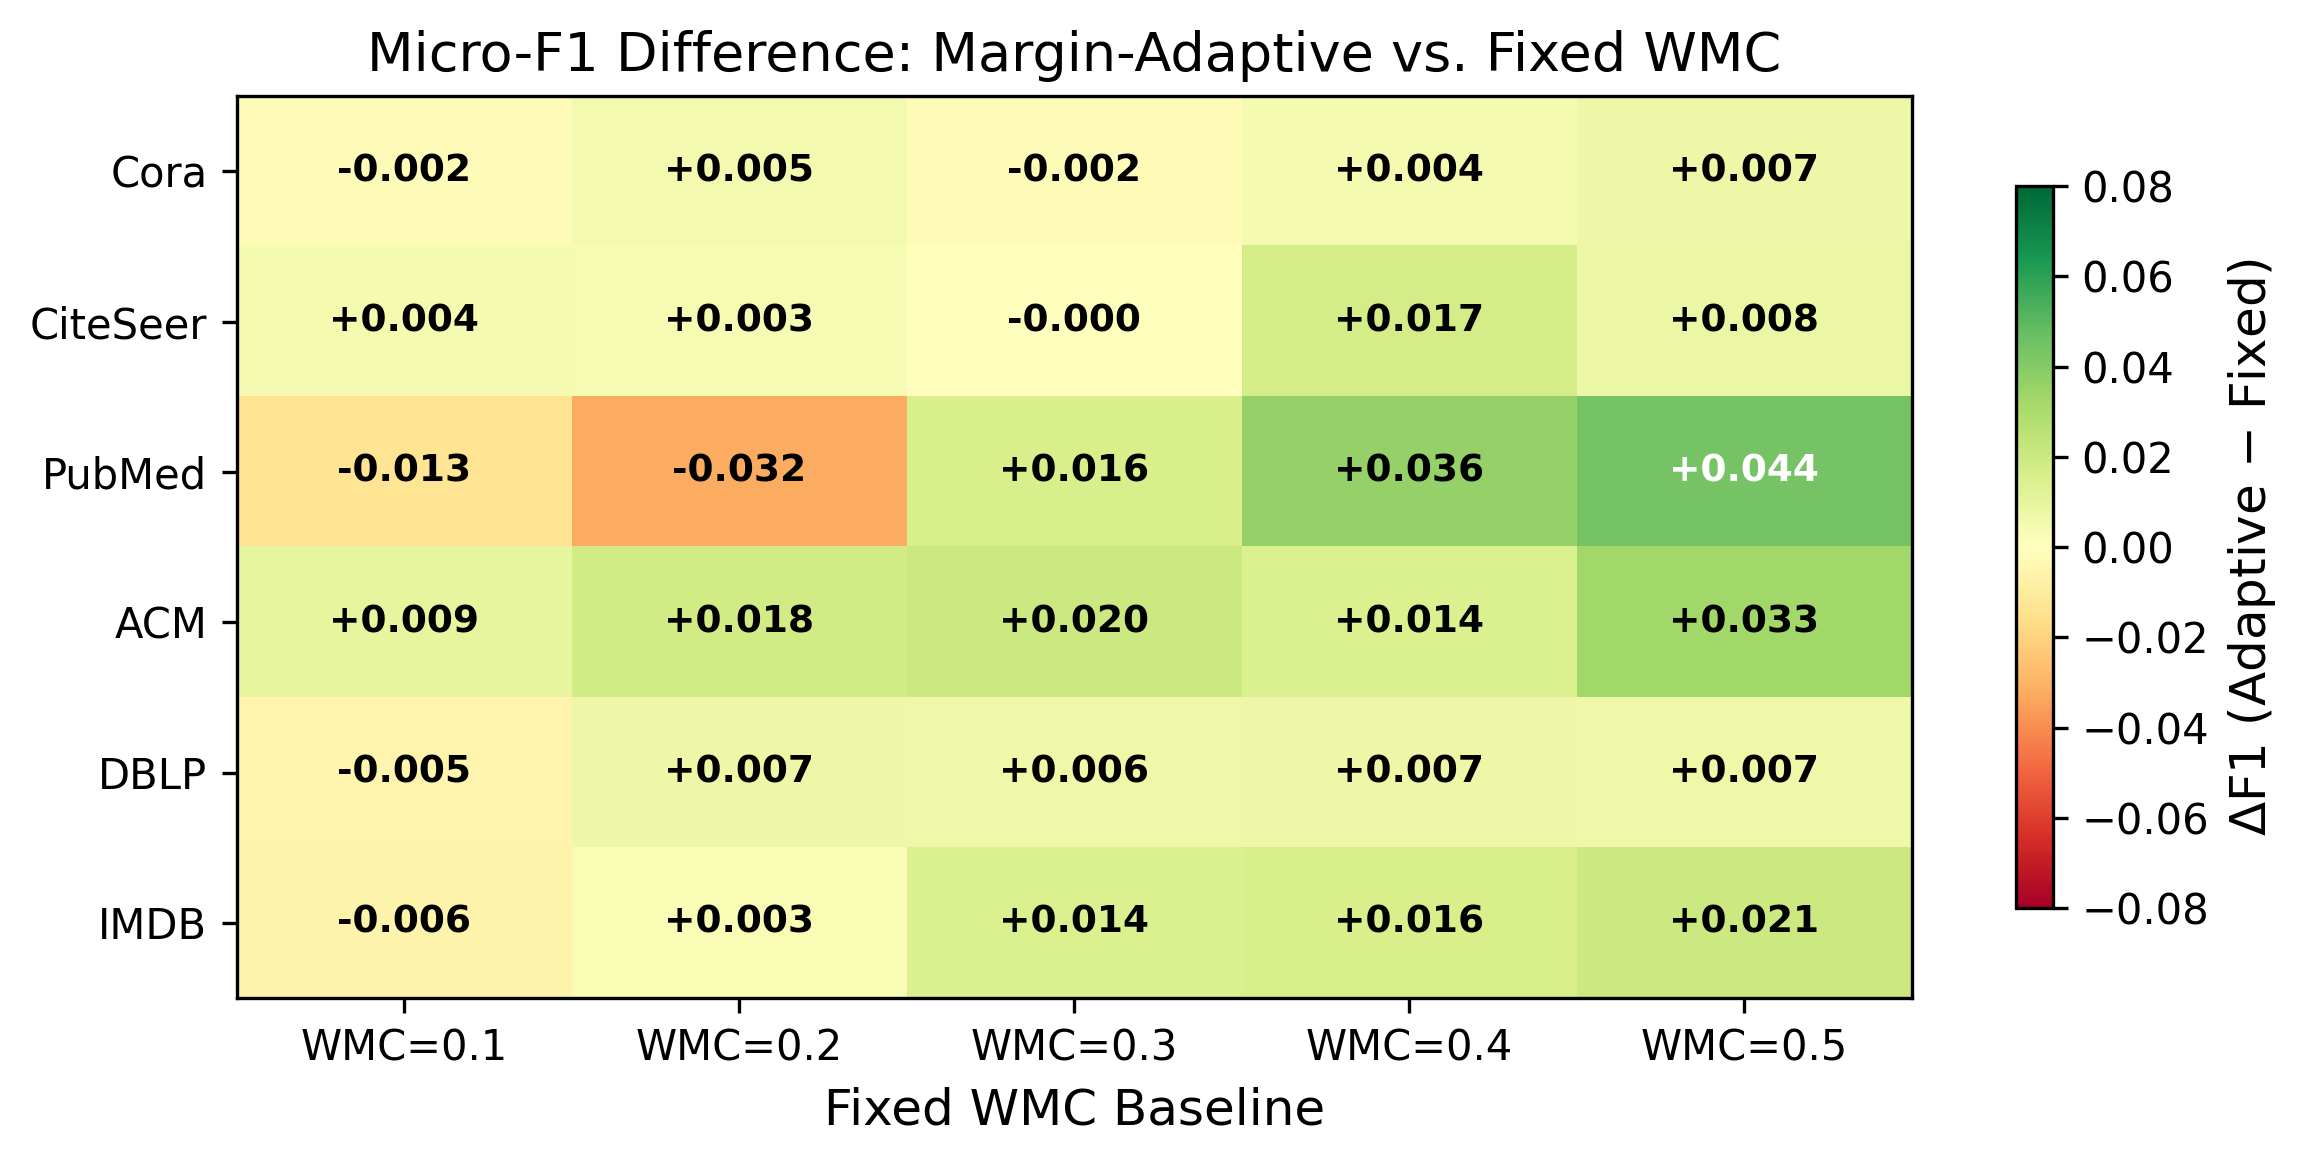
\includegraphics[width=0.65\textwidth]{figures/significance_heatmap.png}
\caption{Micro-F1 difference between Margin-Adaptive and each fixed WMC baseline. Green cells indicate adaptive wins; red cells indicate fixed wins. Margin-Adaptive is competitive with most fixed WMC values across datasets without tuning.}
\label{fig:heatmap}
\end{figure}

\clearpage

\subsubsection{Ambiguity Analysis}
\label{sec:ambiguity-analysis}

\paragraph{Dataset Ambiguity Statistics.}

Table~\ref{tab:ambiguity-stats} presents the membership ambiguity statistics derived from DANMF output across all datasets.

\begin{table}[ht]
\centering
\caption{Membership ambiguity statistics per dataset (DANMF output, WMC~=~0.30 overlap).}
\label{tab:ambiguity-stats}
\begin{tabular}{lcccccc}
\toprule
\textbf{Dataset} & \textbf{Entropy~$\mu$} & \textbf{Entropy~$\sigma$} & \textbf{Ambiguity~$\mu$} & \textbf{Overlap Ratio} & \textbf{Mean Clusters/Node} \\
\midrule
Cora      & 0.138 & 0.167 & 0.305 & 0.279 & 1.37 \\
CiteSeer  & 0.071 & 0.126 & 0.467 & 0.137 & 1.15 \\
PubMed    & 0.143 & 0.166 & 0.187 & 0.230 & 1.27 \\
ACM       & 0.159 & 0.190 & 0.256 & 0.240 & 1.26 \\
DBLP      & 0.122 & 0.173 & 0.522 & 0.211 & 1.24 \\
IMDB      & 0.419 & 0.280 & 0.500 & 0.621 & 2.20 \\
\bottomrule
\end{tabular}
\end{table}

IMDB has the highest entropy ($\mu = 0.419$) and overlap ratio (0.621), reflecting its dense structure and role-heterogeneous nature.
CiteSeer has the lowest entropy ($\mu = 0.071$), indicating near-deterministic memberships.
Entropy variance is highest on IMDB ($\sigma = 0.280$) and lowest on CiteSeer ($\sigma = 0.126$), suggesting that IMDB has the widest spread of ambiguity levels---the condition under which adaptive thresholding should have the most room to help.

\paragraph{Correlation Between Ambiguity and Overlap.}

Table~\ref{tab:correlations} reports Spearman rank correlations between ambiguity measures and structural properties.
All correlations are significant at $p < 0.001$.

\begin{table}[ht]
\centering
\caption{Spearman rank correlations between ambiguity measures and structural properties.}
\label{tab:correlations}
\begin{tabular}{lcccc}
\toprule
\textbf{Dataset} & \textbf{Entropy$\leftrightarrow$Overlap} & \textbf{Entropy$\leftrightarrow$Clusters} & \textbf{Ambiguity$\leftrightarrow$Overlap} & \textbf{Entropy$\leftrightarrow$Ambiguity} \\
\midrule
Cora      & 0.706 & 0.716 & 0.600 & 0.528 \\
CiteSeer  & 0.601 & 0.602 & 0.097 & $-$0.366 \\
PubMed    & 0.693 & 0.697 & 0.729 & 0.981 \\
ACM       & 0.696 & 0.698 & 0.613 & 0.624 \\
DBLP      & 0.677 & 0.680 & 0.099 & $-$0.398 \\
IMDB      & 0.701 & 0.808 & 0.790 & 0.676 \\
\bottomrule
\end{tabular}
\end{table}

Entropy correlates strongly with both overlap assignment and cluster count across all datasets ($r = 0.60$--$0.81$), confirming that high-entropy nodes are systematically assigned to more clusters.
Ambiguity correlates strongly with overlap on four of six datasets but weakly on CiteSeer and DBLP ($r \approx 0.10$), where entropy and margin measure fundamentally different aspects of the membership distribution.
On PubMed, entropy and ambiguity are nearly identical ($r = 0.981$), suggesting the two measures are redundant on that dataset.

%The scatter plots in Figure~\ref{fig:entropy-vs-clusters} visualize the entropy--cluster count relationship across all datasets, showing the clear positive trend.
%
%\begin{figure}[ht]
%\centering
%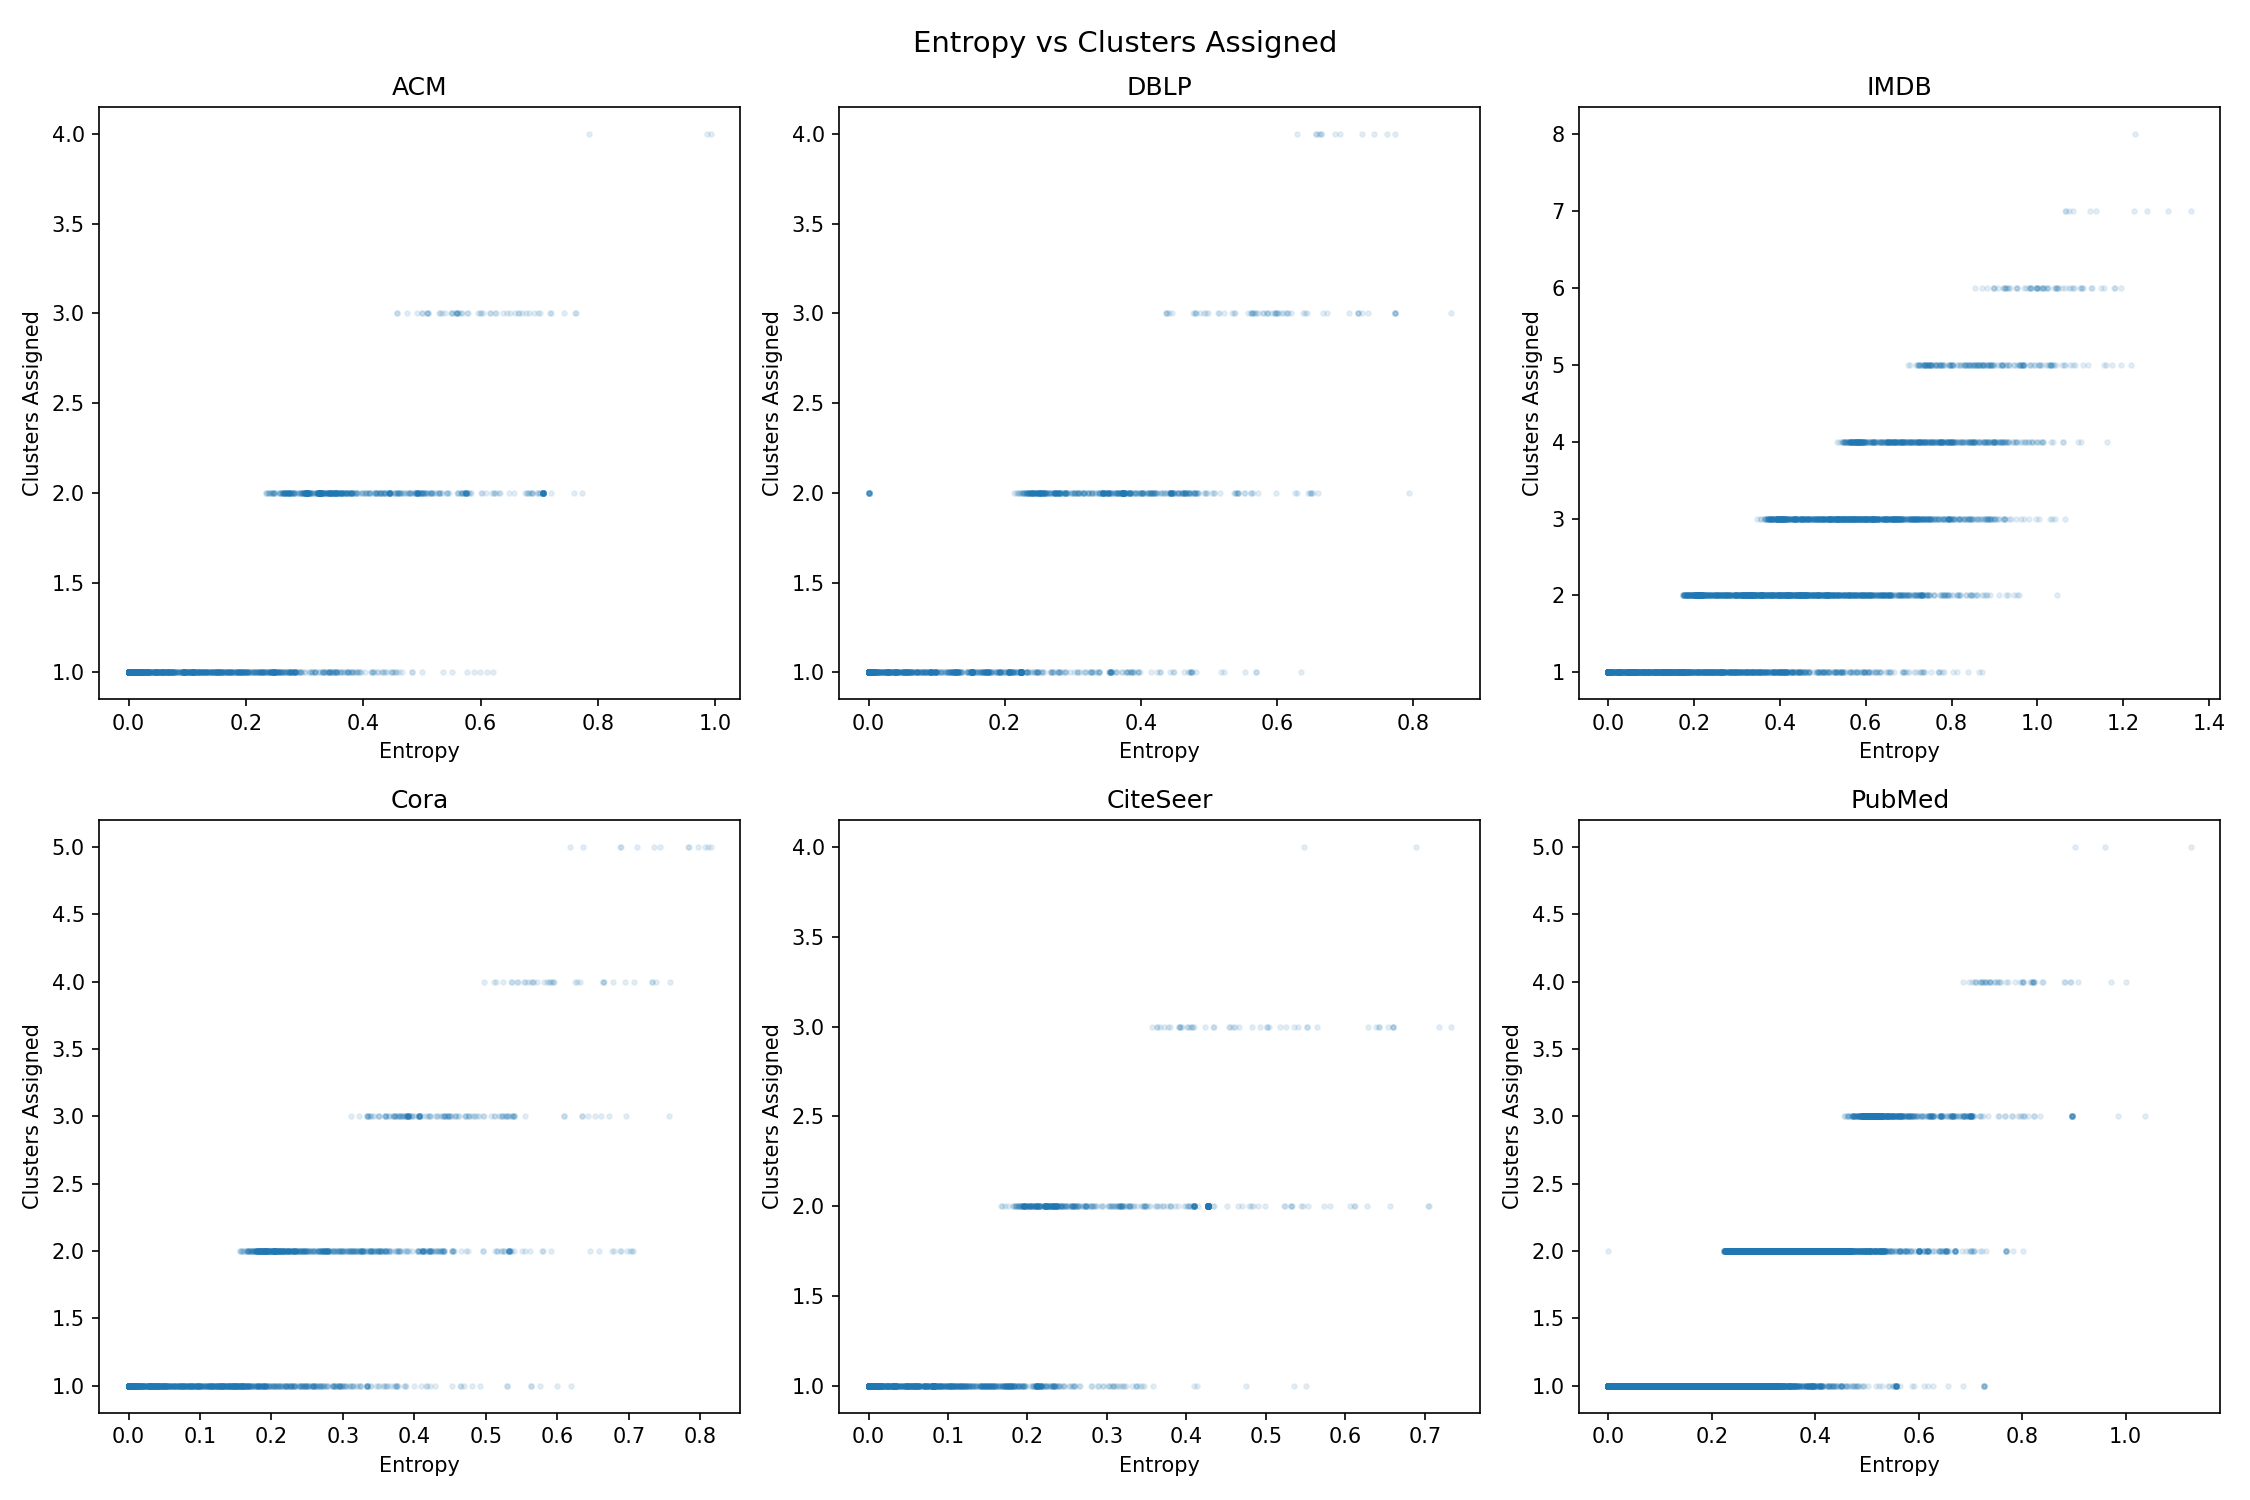
\includegraphics[width=\textwidth]{figures/entropy_vs_clusters.png}
%\caption{Entropy vs.\ number of clusters assigned for each dataset. Each point represents a node. Higher entropy correlates with more cluster assignments, confirming that entropy captures genuine membership ambiguity.}
%\label{fig:entropy-vs-clusters}
%\end{figure}

\paragraph{Stratified Ambiguity Analysis.}

To directly test the ambiguity hypothesis, we stratify nodes into entropy terciles and examine their overlap assignment rates.
Table~\ref{tab:stratified} presents the results.

\begin{table}[ht]
\centering
\caption{Overlap ratio and mean clusters per entropy tercile.}
\label{tab:stratified}
\begin{tabular}{lllcccc}
\toprule
\textbf{Dataset} & \textbf{Tercile} & \textbf{Entropy Range} & \textbf{Nodes} & \textbf{Overlap Ratio} & \textbf{Mean Clusters} \\
\midrule
\multirow{3}{*}{Cora}
  & Low    & 0--0.0001    & 903  & 0.000 & 1.00 \\
  & Medium & 0.0001--0.19 & 902  & 0.076 & 1.08 \\
  & High   & 0.19--0.81   & 903  & 0.761 & 2.04 \\
\midrule
\multirow{2}{*}{CiteSeer}
  & Low+Med & 0--0.03     & 2218 & 0.000 & 1.00 \\
  & High    & 0.03--0.73  & 1109 & 0.411 & 1.46 \\
\midrule
\multirow{3}{*}{PubMed}
  & Low    & 0--0.009     & 6570 & 0.000 & 1.00 \\
  & Medium & 0.009--0.20  & 6575 & 0.000 & 1.00 \\
  & High   & 0.20--1.13   & 6572 & 0.689 & 1.80 \\
\midrule
\multirow{3}{*}{ACM}
  & Low    & 0--0.005     & 788  & 0.000 & 1.00 \\
  & Medium & 0.005--0.23  & 787  & 0.000 & 1.00 \\
  & High   & 0.23--0.99   & 788  & 0.718 & 1.79 \\
\midrule
\multirow{2}{*}{DBLP}
  & Low+Med & 0--0.15     & 1727 & 0.006 & 1.01 \\
  & High    & 0.15--0.86  & 864  & 0.620 & 1.72 \\
\midrule
\multirow{3}{*}{IMDB}
  & Low    & 0--0.26      & 1544 & 0.170 & 1.17 \\
  & Medium & 0.26--0.56   & 1542 & 0.739 & 2.02 \\
  & High   & 0.56--1.36   & 1544 & 0.953 & 3.42 \\
\bottomrule
\end{tabular}
\end{table}

The pattern is consistent across all datasets: high-entropy nodes receive 41--95\% overlap assignment, while low-entropy nodes receive 0--17\%.
On IMDB, the most ambiguous nodes are assigned to 3.4 clusters on average, confirming they genuinely straddle multiple communities.
On CiteSeer and DBLP, where many nodes have near-zero entropy, the two lowest terciles merge into a single low-entropy bin with almost no overlap.
Figure~\ref{fig:overlap-by-tercile} visualizes this relationship, showing the stark contrast between entropy terciles.

\begin{figure}[ht]
\centering

\includegraphics[width=\textwidth]{figures/overlap_vs_entropy.png}
\caption{Overlap ratio by entropy tercile for each dataset. High-entropy nodes consistently receive far more overlap assignments than low-entropy nodes, validating the hypothesis that membership ambiguity identifies useful overlap candidates.}
\label{fig:overlap-by-tercile}
\end{figure}

\paragraph{Why Adaptive WMC Helps Some Datasets More Than Others.}

Table~\ref{tab:gains-vs-variance} examines the relationship between entropy statistics and adaptive performance gain.

\begin{table}[ht]
\centering
\caption{Relationship between entropy statistics and adaptive performance gain.}
\label{tab:gains-vs-variance}
\begin{tabular}{llll}
\toprule
\textbf{Dataset} & \textbf{Entropy Variance} & \textbf{Gain vs.\ Default (F1 pts)} & \textbf{Interpretation} \\
\midrule
ACM      & 0.036 & +2.0 & Many ambiguous nodes; largest absolute gain \\
PubMed   & 0.027 & +1.6 & High variance $\rightarrow$ many ambiguous nodes $\rightarrow$ large gain \\
IMDB     & 0.079 & +1.4 & Highest mean + variance $\rightarrow$ largest overlap ratios \\
DBLP     & 0.030 & +1.2 & Moderate variance $\rightarrow$ modest gain \\
Cora     & 0.028 & $-$0.2 & Near-optimal default $\rightarrow$ no room regardless of method \\
CiteSeer & 0.016 & +0.0 & Very low entropy $\rightarrow$ minimal room for improvement \\
\bottomrule
\end{tabular}
\end{table}

Performance gains from adaptive thresholding show a partial relationship with entropy variance: the largest gains occur on datasets with higher variance (ACM, PubMed, IMDB), while CiteSeer, with the lowest variance, gains nothing.
The relationship is not strictly monotonic---variance alone does not determine the gain, because the benefit also depends on how far the default WMC~=~0.30 is from the per-dataset optimum.
For example, Cora (variance~0.028) shows negligible gain because WMC~=~0.30 is already the best fixed threshold (0.832 micro F1), leaving no room for improvement regardless of method.
PubMed and DBLP have similar entropy variance to Cora ($\sigma^2 \approx 0.03$), yet gain +1.6 and +1.2 F1, respectively, because their default WMC~=~0.30 underperforms the per-dataset optimum (WMC~=~0.20 for PubMed, WMC~=~0.10 for DBLP), and adaptive methods can lower the threshold for ambiguous nodes to recover the lost performance.
The dashed trend line in Figure~\ref{fig:gain-variance} shows the linear fit between entropy variance and performance gain, illustrating the overall positive association despite the outliers.
Figure~\ref{fig:gain-variance} visualizes this relationship.

\begin{figure}[ht]
\centering
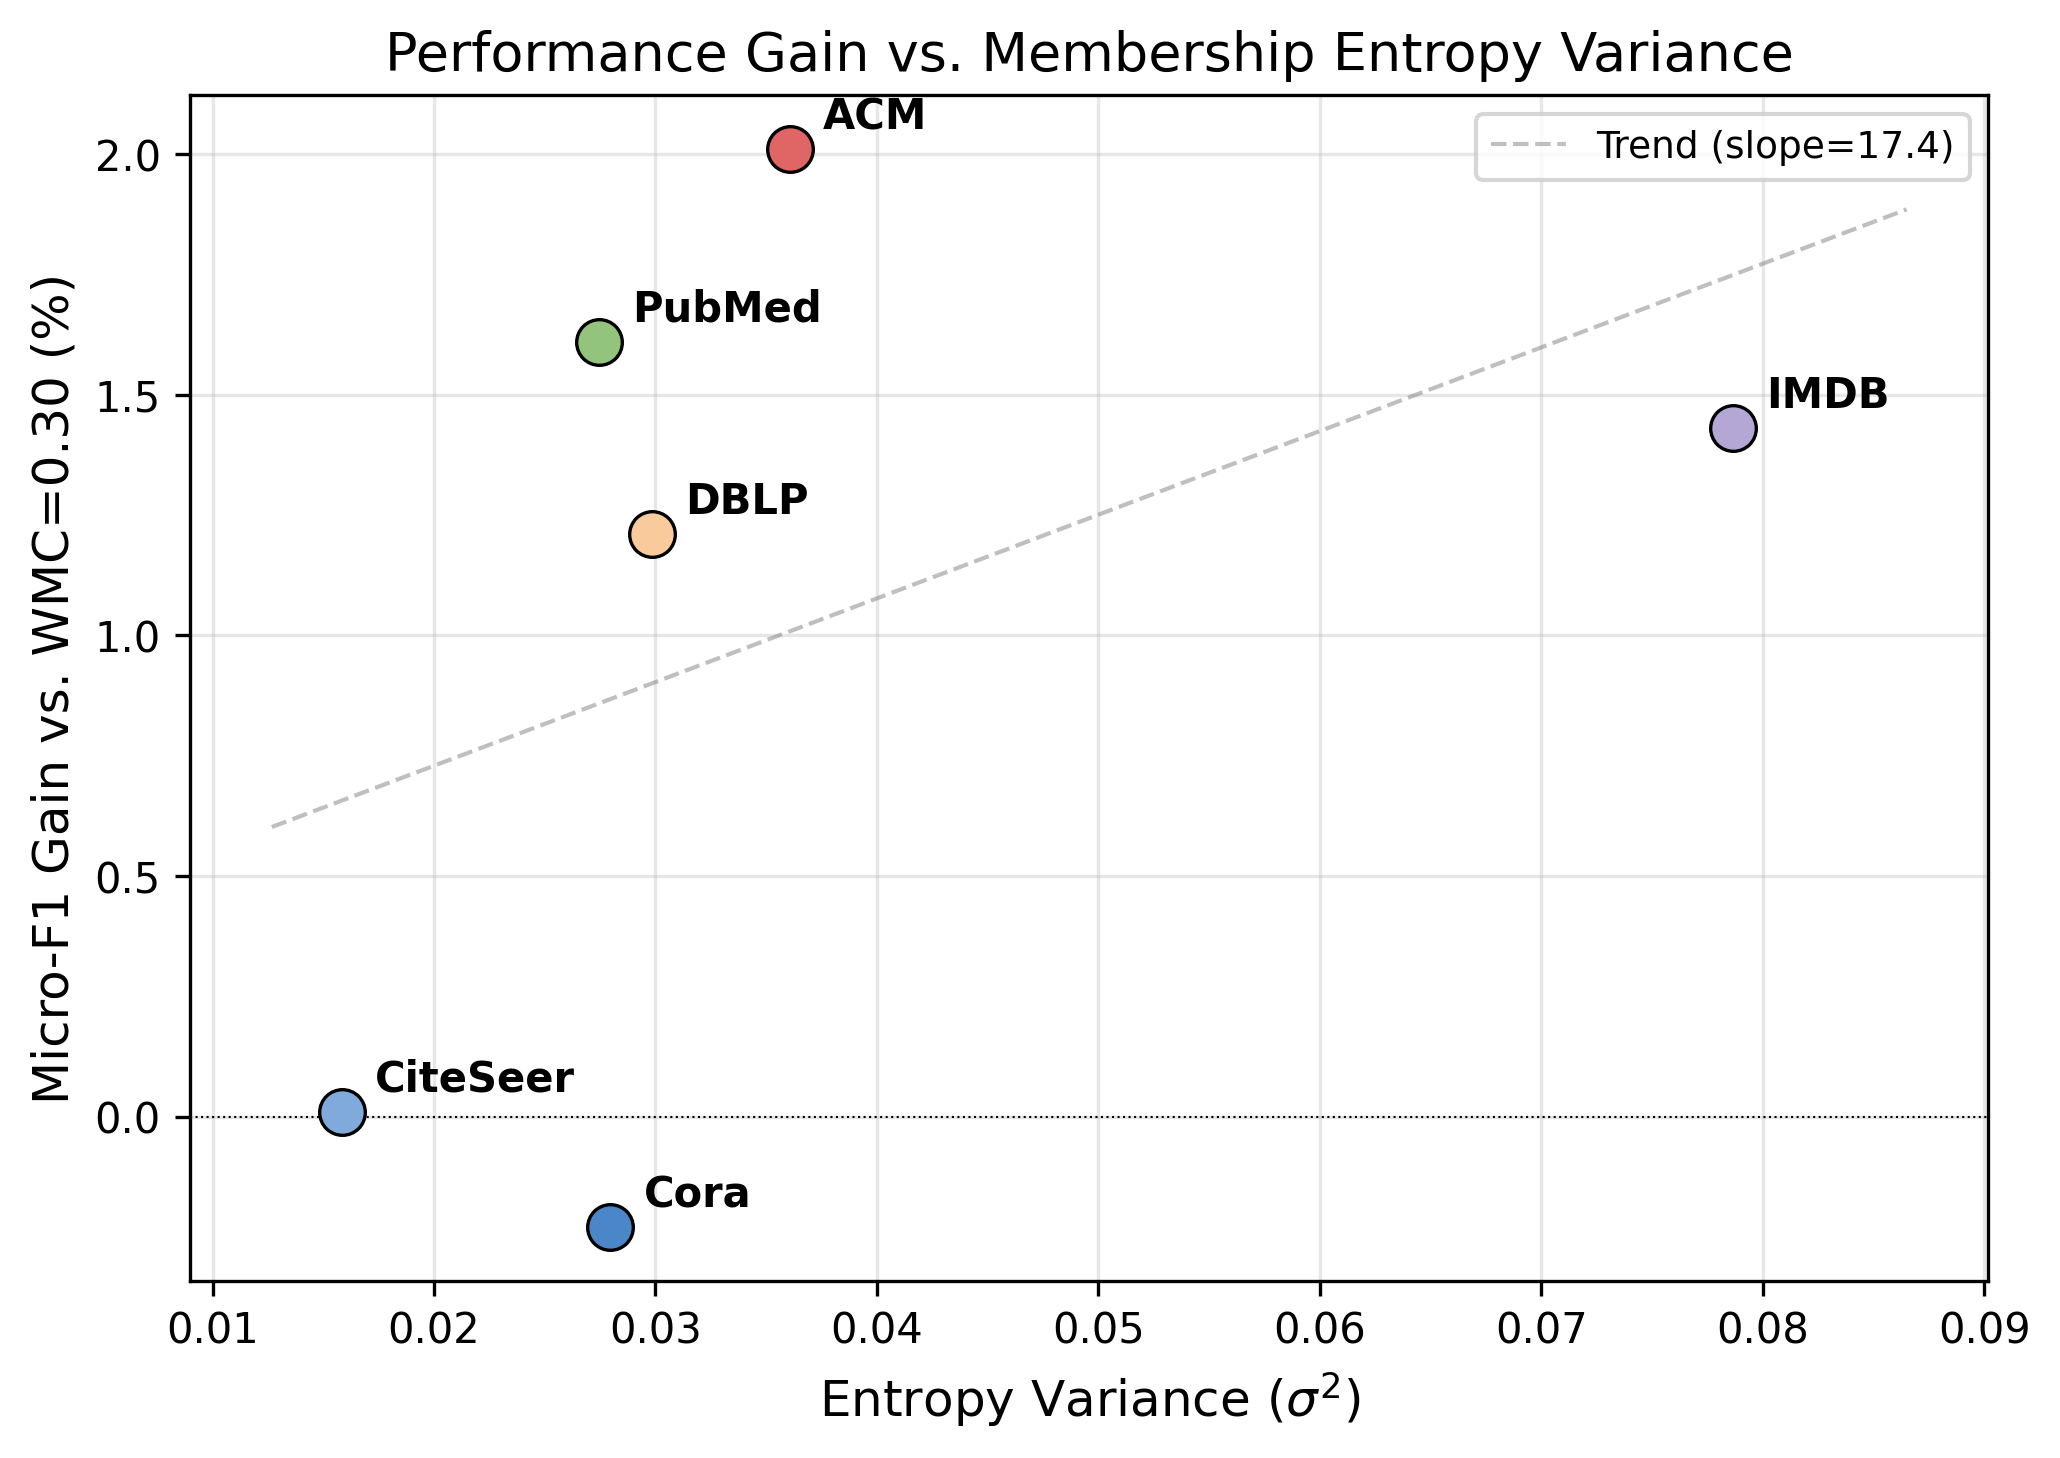
\includegraphics[width=0.75\textwidth]{figures/gain_vs_variance.png}
\caption{Performance gain (micro-F1 improvement over WMC~=~0.30) vs.\ entropy variance ($\sigma^2$) for each dataset. Datasets with higher entropy variance (ACM, PubMed, IMDB) show the largest gains, while CiteSeer, with the lowest variance, gains nothing.}
\label{fig:gain-variance}
\end{figure}

Ceiling effects (ACM), near-optimal defaults (Cora), and very low ambiguity (CiteSeer) limit gains regardless of variance.

%%======================================================================
\section{Discussion}
\label{sec:discussion}
%%======================================================================

This section interprets the experimental findings, discusses their implications, and outlines limitations and future directions.
We first validate the ambiguity hypothesis and the practical value of eliminating the WMC hyperparameter (Sections~\ref{sec:discussion}-\ref{subsec:agnosticism}), followed by practical recommendations (Section~\ref{subsec:recommendations}) and threats to validity (Section~\ref{sec:threats}).

\subsection{The Ambiguity Hypothesis Is Validated}

The stratified analysis and correlation studies provide strong evidence that community-membership ambiguity identifies useful overlap nodes.
High-entropy nodes are 41--95\% overlap candidates, and they are assigned to 1.5--3.4 clusters on average.
The mechanism is intuitive: nodes with ambiguous memberships genuinely participate in multiple communities, and including them in multiple cluster subgraphs provides the GCN with richer training signals.
Low-entropy nodes, by contrast, are well-served by single-cluster training.

\subsection{Adaptive Thresholding Eliminates a Hyperparameter}

The primary practical contribution is the elimination of the WMC hyperparameter search.
Our fixed-WMC comparison (Table~\ref{tab:main-results}) shows that the optimal WMC varies across datasets: WMC~=~0.30 is best for Cora and CiteSeer, WMC~=~0.20 for PubMed, and WMC~=~0.10 for DBLP and IMDB (and no overlap at all on ACM).
Without adaptive methods, practitioners must search over WMC values---a costly process that requires retraining on each dataset.
Margin-Adaptive (or the Hybrid) with $\lambda = 0.50$ achieves competitive performance across all six datasets without per-dataset tuning, and is significantly better than the fixed default in the pooled paired analysis ($p=0.022$).
Importantly, this is not a claim of universal superiority over well-tuned baselines, but rather a demonstration that a single universal configuration ($\mathrm{WMC}_{\mathrm{base}} = 0.3$, $\lambda = 0.5$) performs comparably to per-dataset tuned WMC, eliminating the need for grid search.
This is particularly valuable in scenarios where practitioners work with many graphs or where the optimal WMC is not known a priori.
Furthermore, while $\lambda$ is technically a hyperparameter, it acts as a global robustness knob rather than a dataset-specific threshold.
As shown in the ablation study (Tables~\ref{tab:entropy-lambda},~\ref{tab:margin-lambda}, and~\ref{tab:hybrid-lambda}), setting $\lambda = 0.50$ consistently yields near-optimal or optimal results across all six diverse datasets without any per-dataset tuning.
This contrasts sharply with the fixed WMC baseline, where the optimal value varies drastically across datasets (e.g., 0.10 for DBLP/IMDB vs.~0.30 for Cora/CiteSeer).
The sensitivity to $\lambda$ is substantially lower than the sensitivity to WMC, thus practically eliminating the need for a grid search.

\subsection{Performance Gains Are Modest but Real}

At matched overlap ratios, adaptive methods improve by +0.003 to +0.018 F1 over fixed baselines on four of six datasets.

The gains are real but modest, reflecting the fact that the original WMC already captures a substantial portion of the useful overlap signal.
Adaptive methods refine this signal by scaling the threshold based on node-level ambiguity, but the marginal improvement is bounded.
The contribution is not universal performance superiority over well-tuned baselines, but rather principled threshold selection that eliminates the tuning cost.

\subsection{Entropy vs.\ Margin: Complementary Signals}

Entropy-Adaptive, Margin-Adaptive, and the Hybrid variant perform similarly overall, but show different per-dataset preferences.
On datasets where ambiguity is primarily a top-two competition, Margin-Adaptive performs best with light adaptation on DBLP ($\lambda = 0.25$) and moderate adaptation on CiteSeer ($\lambda = 0.50$).
On datasets with richer multi-cluster ambiguity (PubMed, IMDB), stronger adaptation ($\lambda = 0.75$) helps all variants.
The weak correlation between entropy and ambiguity on DBLP and CiteSeer ($r \approx -0.4$) confirms that these measures capture genuinely different aspects of the membership distribution.
The Hybrid variant combines both signals and achieves the best overall result on DBLP, confirming their complementarity.

\subsection{Community-Detection Agnosticism}
\label{subsec:agnosticism}

While DANMF was utilized in this study to generate the soft membership matrix $P$, the proposed adaptive thresholding mechanism is fundamentally agnostic to the underlying community detection algorithm.
As long as the chosen clustering method outputs a normalized membership matrix $P \in \mathbb{R}^{N \times K}$ whose rows sum to one, the adaptive WMC formulas (Entropy, Margin, and Hybrid) can be applied directly without any modification.
This makes Adaptive-OCGCN a general-purpose plugin that can improve partition-based GNN training pipelines utilizing various soft clustering techniques.

\subsection{Practical Recommendations}
\label{subsec:recommendations}

Based on our findings, we recommend:

\begin{enumerate}
  \item {Default configuration:} Margin-Adaptive (or the Hybrid) with $\mathrm{WMC}_{\mathrm{base}} = 0.3$ and $\lambda = 0.50$. This single configuration is significantly better than the fixed default in the pooled paired analysis ($p=0.022$), outperforms it on four of six datasets, and provides competitive performance across all tested datasets without per-dataset tuning.
  \item {When strong ambiguity is expected:} Increase $\lambda$ to 0.75 (as on IMDB).
  \item {When a tuned fixed WMC is available:} Adaptive methods are unlikely to significantly outperform it, but they provide a principled starting point that avoids the tuning cost.
\end{enumerate}

\subsection{Threats to Validity}
\label{sec:threats}

\paragraph{Dataset scope.}
We evaluate on six datasets, all of moderate size (2,363--19,717 nodes).
The largest graph, PubMed, has 19,717 nodes, which is relatively small by modern GNN standards, even though the paper title emphasizes scalable GNNs.
It is crucial, however, to distinguish between the scalability of the proposed adaptive thresholding mechanism and the scalability of the upstream clustering algorithm.
The adaptive WMC framework itself is theoretically highly scalable: the node-level ambiguity scores add only $O(NK)$ or $O(NK \log K)$ computational overhead, which is negligible compared with GCN training.
The current evaluation is limited to standard benchmark sizes because the upstream dependency---specifically the DANMF clustering algorithm used to generate $P$---becomes a computational bottleneck on graphs with millions of nodes.
Therefore, the proposed method is fully prepared for large-scale graphs, provided it is paired with a more scalable soft community detection algorithm in future work.
Scaling to larger graphs (e.g., OGB benchmarks with millions of nodes) would further strengthen the claims and test whether the ambiguity signal remains informative at scale.

\paragraph{Community detection method.}
All experiments use DANMF for membership estimation.
Different community detection methods may produce different membership distributions, potentially affecting the ambiguity signal.
The adaptive framework is method-agnostic in principle, but the specific entropy and margin values depend on the quality of the membership estimation.
On PubMed, DANMF yields a highly imbalanced partition (the largest cluster contains about 62\% of the nodes), which degrades the cluster-based no-overlap baseline (0.521 micro F1) below a random-partition control (0.852); the adaptive overlap methods still recover substantial accuracy (0.628) in this regime.
This is a limitation of the clustering step rather than of overlap selection, and it suggests that balancing cluster sizes (e.g., via size constraints or a different $K$) is a promising avenue for future work.

\paragraph{Overlap ratio range.}
Our experiments fix $\mathrm{WMC}_{\mathrm{base}} = 0.3$ and vary only $\lambda$.
Different base WMC values could shift the overlap ratio range and affect the relative advantage of adaptive methods.
We chose $\mathrm{WMC}_{\mathrm{base}} = 0.3$ because it is the default in the original OCGCN.

\paragraph{Statistical power.}
With 20 seeds per configuration in the main comparison (10 in the ablation), we detected a significant pooled improvement of Margin-Adaptive over the default threshold ($p = 0.022$).
Non-significant per-dataset differences on Cora, PubMed, and ACM could still reflect limited power to detect small effect sizes; larger-scale experiments with more seeds would clarify this.

\paragraph{Single GCN architecture.}
We use a fixed GCN with 16 hidden units per layer.
Different architectures (deeper/wider GCNs, attention-based models) might interact differently with overlap assignment.
The adaptive thresholding is architecture-agnostic, but the magnitude of its benefit may vary.

\subsection{Conclusion}
\label{sec:conclusion}

This paper introduces adaptive overlap thresholding for Overlapping Cluster-GCN, replacing the global WMC threshold with node-specific thresholds derived from community-membership ambiguity.
Three variants are proposed: Entropy-Adaptive WMC, which scales the threshold by normalized membership entropy, Margin-Adaptive WMC, which scales by the ambiguity of the top-two membership gap, and Hybrid-Adaptive WMC, which combines both signals.
All three replace per-dataset WMC grid search with a single universal configuration ($\mathrm{WMC}_{\mathrm{base}} = 0.3$, $\lambda = 0.5$) that achieves competitive performance across six benchmark graphs; Margin-Adaptive is significantly better than the fixed default in the pooled paired analysis ($p=0.022$).

The core hypothesis---that membership ambiguity identifies useful overlap nodes---is validated through stratified analysis showing that high-entropy nodes are 41--95\% overlap candidates, with strong correlations between entropy and cluster count on all datasets.
Performance gains from adaptive thresholding are modest but real: at matched overlap ratios, adaptive methods improve by +0.003 to +0.018 F1 over fixed baselines on four of six datasets, and Margin-Adaptive is significantly better than the fixed default in the pooled paired analysis ($p=0.022$).

The practical value of adaptive thresholding is the removal of the WMC hyperparameter search, a process that varies across datasets and requires costly retraining.
Margin-Adaptive (or the Hybrid) with $\lambda = 0.50$ provides a robust default that works well across diverse graph types.
Future work should explore scaling to larger graphs, per-node $\lambda$ adaptation, and theoretical analysis of the overlap quality bound.

%%======================================================================
%% References
%%======================================================================

\bibliography{sn-bibliography}% common bib file
%% if required, the content of .bbl file can be included here once bbl is generated
%%\input sn-article.bbl

\section*{Statements \& Declarations}

\subsection*{Funding}
The authors declare that no funds, grants, or other support were received during the preparation of this manuscript.

\subsection*{Competing Interests}
The authors have no relevant financial or non-financial interests to disclose.

\subsection*{Declaration of Generative AI and AI-assisted Technologies in the Writing Process}

During the preparation of this work, the author used AI-assisted tools and services, including Mimo and Buffy (via Freebuff) and DeepSeek for various aspects of the research and manuscript preparation process, including writing and editing assistance, code development, experimental design and execution, data analysis, figure and table preparation, manuscript organization, and scientific presentation. All generated content and outputs were reviewed, verified, and edited by the author as appropriate. The author takes full responsibility for the accuracy, integrity, and final content of the publication.


\end{document}
